% Spacing Setup
\setlength{\parskip}{6pt}
\setlength{\parindent}{0pt}
\usetikzlibrary{arrows.meta}
% TikZ Predetermined Elements 
\tikzset{
    coil spring/.pic={
        % Parameters: length of straight lines and coil
        \def\Lbefore{0.5}   % length of line before coil
        \def\Lafter{0.5}    % length of line after coil
        \def\coilLength{1}  % length of the coil itself

        % Draw left line
        \draw (0,0) -- (\Lbefore,0);

        % Draw coil in the middle
        \draw[decorate, decoration={coil, aspect=0.5, segment length=2mm, amplitude=2mm}]
        (\Lbefore,0) -- (\Lbefore+\coilLength,0);


        % Draw right line
        \draw (\Lbefore+\coilLength,0) -- (\Lbefore+\coilLength+\Lafter,0);
    },
    damper/.pic={
        % The damper drawing
        \draw (0,0) -- (1.4,0);          
        \draw (1.4,-0.2) -- (1.4,0.2);  
        \draw (1.7,0.3) -- (1.7,-0.3) -- (1,-0.3);
        \draw (1.7,0.3) -- (1,0.3);  
        \draw (1.7,0) -- (2.8,0);       
    },
    curvedarrow/.pic={
        \draw[<-, line width=1pt] (30:1cm) arc[start angle=30, end angle=100, radius=1cm];
    },
}

% Problem 16
\newpage

\noindent\rule{\textwidth}{1pt}
\noindent\textbf{Problem 16} \hfill
\\ Determine the transfer function \(H(s) = \frac{\theta_2(s)}{T(s)}\)

\begin{figure}[!ht]
\centering
\resizebox{1\textwidth}{!}{%
\begin{tikzpicture}[scale=1.4, transform shape, font=\large]

    % walls
    \draw[pattern=bricks] (-5.8,-1.5) rectangle (-5,2);     
    \draw[pattern=bricks] (16.8,-1.5) rectangle (16,2);       

    % j1
    \draw (0,0) ellipse (0.5cm and 1cm);  
    \draw (0,1) -- (4,1);                 
    \draw (0,-1) -- (4,-1);               
    \draw (4,1) arc[start angle=90, end angle=-90, x radius=0.5cm, y radius=1cm]; 
    \node at (2.3,0) {$5kg-m^2$};

    % j2
    \draw (8,0) ellipse (0.5cm and 1cm);  
    \draw (8,1) -- (12,1);                 
    \draw (8,-1) -- (12,-1);               
    \draw (12,1) arc[start angle=90, end angle=-90, x radius=0.5cm, y radius=1cm]; 
    \node at (10.4,0) {$3kg-m^2$};
    
    % t1
    \draw[->, thick, color=cyan] (2.3,-1.3) arc[start angle=290, end angle=45, x radius=0.5cm, y radius=1.5cm];
    \node at (2.3,2) {$\theta_1$};
    
     % t2
    \draw[->, thick, color=cyan] (10.8,-1.3) arc[start angle=290, end angle=45, x radius=0.5cm, y radius=1.5cm];
    \node at (10.8,2) {$\theta_2$};
    
    % torque
    \draw[->, thick, color=cyan] (9.8,-1.3) arc[start angle=290, end angle=45, x radius=0.5cm, y radius=1.5cm];
    \node at (9.8,2) {T};

    % fv1
    \pic [scale=1.8] at (-5,0) {damper}; 
    \node at (-2.8,1.2) {8 $N\cdotp m\cdotp s/rad$};

    % fv2
    \pic [scale=1.2] at (4.5,0.4) {damper}; 
    \node at (6,1.4) {1 $N \cdotp m\cdotp s/rad$};

    % fv3
    \pic [scale=1.25] at (12.5,0.4) {damper}; 
    \node at (13.9,1.4) {1 $N \cdotp m\cdotp s/rad$};

    % k1
    \pic [scale=1.75] at (4.4,-0.5) {coil spring};
    \node at (6,-1.2) {9 $N \cdotp m/rad$};

    % k2
    \pic [scale=1.75] at (12.45,-0.5) {coil spring};
    \node at (13.9,-1.2) {3 $N \cdotp m/rad$};

\end{tikzpicture}
}%
\end{figure}

\noindent\rule{\textwidth}{1pt}

\textbf{Given:}
\[
J_1 = 5\ \mathrm{kg\cdot m^2},\quad J_2 = 3\ \mathrm{kg\cdot m^2}
\]
\[
k_1 = 9\ \mathrm{N\cdot m/rad},\quad k_2 = 3\ \mathrm{N\cdot m/rad}
\]
\[
b_1 = 8\ \mathrm{N\cdot m\cdot s/rad},\quad b_2 = 1\ \mathrm{N\cdot m\cdot s/rad},\quad b_3 = 1\ \mathrm{N\cdot m\cdot s/rad}
\]
\[
T(t) \text{ applied at second rotor}
\]
\[
\theta_1(t),\ \theta_2(t)
\]

\textbf{Required:}
\[
\frac{\Theta_2(s)}{T(s)}.
\]

\textbf{Solution:}

Free Body Diagram

\begin{figure}[!ht]
\centering
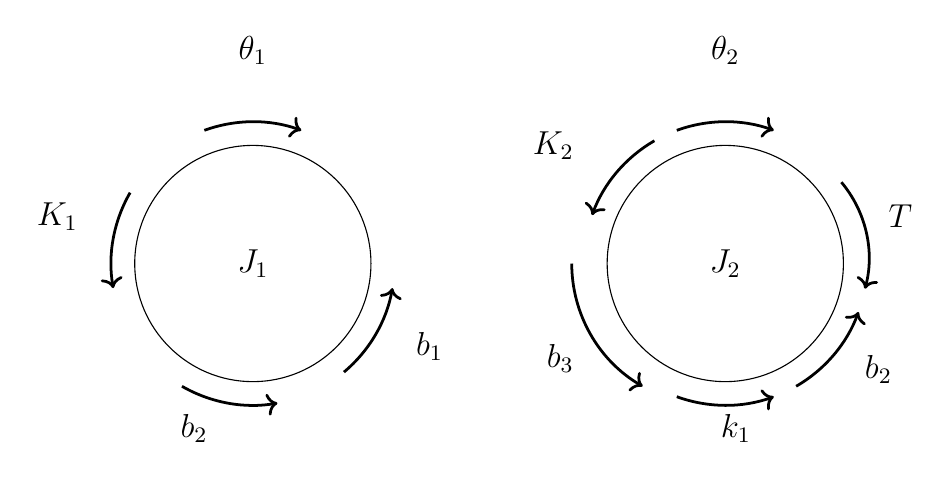
\begin{tikzpicture}[scale=1.5, every node/.style={font=\large}]

    % Circle for J1
    \node[circle, draw, minimum size=3cm] (inertia) at (0,0) {$J_1$};

    % theta1
    \draw[<-, line width=1pt] (70:1.2cm) arc[start angle=70, end angle=110, radius=1.2cm];
    \node at (0,1.8) {$\theta_1$};
    
    % b1 (moved slightly upward-right)
    \draw[->, line width=1pt] (310:1.2cm) arc[start angle=310, end angle=350, radius=1.2cm];
    \node[anchor=west] at (1.3,-0.7) {$b_1$};

    % b2 (kept bottom-left, adjusted outward)
    \draw[->, line width=1pt] (240:1.2cm) arc[start angle=240, end angle=280, radius=1.2cm];
    \node[anchor=east] at (-0.3,-1.4) {$b_2$};
    
    % K1 (adjusted slightly upward-left)
    \draw[->, line width=1pt] (150:1.2cm) arc[start angle=150, end angle=190, radius=1.2cm];
    \node[anchor=east] at (-1.4,0.4) {$K_1$};


\begin{scope}[shift={(4,0)}]

    % Circle for J2
    \node[circle, draw, minimum size=3cm] (inertia) at (0,0) {$J_2$};

    % theta2
    \draw[<-, line width=1pt] (70:1.2cm) arc[start angle=70, end angle=110, radius=1.2cm];
    \node at (0,1.8) {$\theta_2$};
    
    % torque
    \draw[->, line width=1pt] (35:1.2cm) arc[start angle=40, end angle=-15, radius=1cm];
    \node[anchor=west] at (1.3,0.4) {$T$};
    
    % b2
    \draw[->, line width=1pt] (300:1.2cm) arc[start angle=300, end angle=340, radius=1.2cm];
    \node[anchor=west] at (1.1,-0.9) {$b_2$};

    % k1
    \draw[->, line width=1pt] (250:1.2cm) arc[start angle=250, end angle=290, radius=1.2cm];
    \node[anchor=east] at (0.3,-1.4) {$k_1$};

    % b3 
    \draw[->, line width=1pt] (180:1.3cm) arc[start angle=180, end angle=240, radius=1.2cm];
    \node[anchor=east] at (-1.2,-0.8) {$b_3$};

    % k2
    \draw[->, line width=1pt] (120:1.2cm) arc[start angle=120, end angle=160, radius=1.2cm];
    \node[anchor=east] at (-1.2,1.0) {$K_2$};

\end{scope}
\end{tikzpicture}
\end{figure}

Torque balance on Inertia 1:
\[
- D_1 \theta_1 - K_1 (\theta_1 - \theta_2) - D_2 (\theta_1 - \theta_2) = J_1 s^2 \theta_1
\]
\[
-8\theta_1 - 9(\theta_1 - \theta_2) - 1(\theta_1 - \theta_2) = 5s^2 \theta_1
\]
\[
-8\theta_1 - 10\theta_1 + 10\theta_2 = 5s^2 \theta_1
\]
\[
-18\theta_1 + 10\theta_2 = 5s^2 \theta_1
\]
\[
10\theta_2 = (5s^2 + 18)\theta_1 \quad \text{(1)}
\]

Torque balance on Inertia 2:
\[
T(s) - D_3 \theta_2 - K_2 \theta_2 - K_1 (\theta_2 - \theta_1) - D_2 (\theta_2 - \theta_1) = J_2 s^2 \theta_2
\]
\[
T(s) - 1\theta_2 - 3\theta_2 - 9(\theta_2 - \theta_1) - 1(\theta_2 - \theta_1) = 3s^2 \theta_2
\]
\[
T(s) - 4\theta_2 - 10\theta_2 + 10\theta_1 = 3s^2 \theta_2
\]
\[
T(s) + 10\theta_1 - 14\theta_2 = 3s^2 \theta_2
\]
\[
T(s) + 10\theta_1 = (3s^2 + 14)\theta_2 \quad \text{(2)}
\]

Substitute (1) into (2):
\[
T(s) + 10\left( \frac{10\theta_2}{5s^2 + 18} \right) = (3s^2 + 14)\theta_2
\]

\[
T(s) + \frac{100\theta_2}{5s^2 + 18} = (3s^2 + 14)\theta_2
\]

\[
T(s) = \left( 3s^2 + 14 - \frac{100}{5s^2 + 18} \right)\theta_2
\]

\[
\frac{\theta_2(s)}{T(s)} = \frac{1}{3s^2 + 14 - \frac{100}{5s^2 + 18}}
\]

\[
\frac{\theta_2(s)}{T(s)}= \frac{1}{\frac{(3s^2 + 14)(5s^2 + 18) - 100}{5s^2 + 18}}
\]

\[
\frac{\theta_2(s)}{T(s)}= \frac{5s^2 + 18}{(3s^2 + 14)(5s^2 + 18) - 100}
\]

\[
\frac{\theta_2(s)}{T(s)}= \frac{5s^2 + 18}{15s^4 + 54s^2 + 70s^2 + 252 - 100}
\]

\[
\frac{\theta_2(s)}{T(s)}= \frac{5s^2 + 18}{15s^4 + 124s^2 + 152}
\]

\[
\boxed{\frac{\theta_2(s)}{T(s)} = \frac{5s^2 + 18}{15s^4 + 124s^2 + 152}}
\]

% Problem 17
\newpage

\noindent\rule{\textwidth}{1pt}
\noindent\textbf{Problem 17} \hfill
\\ Determine the transfer function \(H(s) = \frac{\theta_3(s)}{T(s)}\)
\begin{figure}[!ht]
\centering
\resizebox{1\textwidth}{!}{%
\begin{tikzpicture}[scale=1.3, transform shape, font=\medium]
    % walls
    \draw[pattern=bricks] (-3.8,-1.5) rectangle (-3,1.5);
    \draw[pattern=bricks] (16.3,-1.5) rectangle (17.1,1.5);

    % fv1
    \pic [scale=1.05] at (-3,0) {damper}; 
    \node at (-1.6,0.9) {8 $N \cdotp m\cdotp s/rad$};

    % fv2
    \pic [scale=0.8] at (3.25,0.4) {damper}; 
    \node at (4.2,1.2) {1 $N \cdotp m\cdotp s/rad$};

    % fv3
    \pic [scale=0.85] at (13.9,0) {damper}; 
    \node at (15,0.8) {2 $N \cdotp m\cdotp s/rad$};

    % k1
    \pic [scale=1.1] at (3.3,-0.4) {coil spring};
    \node at (4.3,-1.1) {9 $N \cdotp m/rad$};

    % k2
    \pic [scale=0.9] at (8.85,0) {coil spring};
    \node at (9.7,-1.3) {7 $N \cdotp m/rad$};
    
    % j1
    \draw (0,0) ellipse (0.3cm and 1cm);  
    \draw (0,1) -- (3,1);                 
    \draw (0,-1) -- (3,-1);               
    \draw (3,1) arc[start angle=90, end angle=-90, x radius=0.3cm, y radius=1cm]; 
    \node at (1.7,0) {2$kg-m^2$};

     % j2
    \draw (5.6,0) ellipse (0.3cm and 1cm);  
    \draw (5.6,1) -- (8.6,1);                 
    \draw (5.6,-1) -- (8.6,-1);               
    \draw (8.6,1) arc[start angle=90, end angle=-90, x radius=0.3cm, y radius=1cm]; 
    \node at (7.3,0) {$3kg-m^2$};

    % j3
    \draw (10.6,0) ellipse (0.3cm and 1cm);  
    \draw (10.6,1) -- (13.6,1);                 
    \draw (10.6,-1) -- (13.6,-1);               
    \draw (13.6,1) arc[start angle=90, end angle=-90, x radius=0.3cm, y radius=1cm]; 
    \node at (12.2,0) {$4kg-m^2$};
    
    % t1
    \draw[->, thick, color=cyan] (2.2,-1.3) arc[start angle=290, end angle=45, x radius=0.5cm, y radius=1.5cm];
    \node at (2.2,2) {$\theta_1$};

    % t2
    \draw[->, thick, color=cyan] (7.5,-1.3) arc[start angle=290, end angle=45, x radius=0.5cm, y radius=1.5cm];
    \node at (7.5,2) {$\theta_2$};

    % t3
    \draw[->, thick, color=cyan] (12.5,-1.3) arc[start angle=290, end angle=45, x radius=0.5cm, y radius=1.5cm];
    \node at (12.5,2) {$\theta_3$};
    
    % torque
    \draw[->, thick, color=cyan] (1.3,-1.3) arc[start angle=290, end angle=45, x radius=0.5cm, y radius=1.5cm];
    \node at (1.3,2) {$T$};

\end{tikzpicture}
}%
\end{figure}

\noindent\rule{\textwidth}{1pt}
\textbf{Given:}
\[
J_1 = 2\ \mathrm{kg\cdot m^2},\quad 
J_2 = 3\ \mathrm{kg\cdot m^2},\quad 
J_3 = 4\ \mathrm{kg\cdot m^2}
\]
\[
k_1 = 9\ \mathrm{N\cdot m/rad},\quad 
k_2 = 7\ \mathrm{N\cdot m/rad}
\]
\[
b_1 = 8\ \mathrm{N\cdot m\cdot s/rad},\quad 
b_2 = 1\ \mathrm{N\cdot m\cdot s/rad},\quad 
b_3 = 2\ \mathrm{N\cdot m\cdot s/rad}
\]
\[
T(t) \text{ applied at first rotor}
\]
\[
\theta_1(t),\quad \theta_2(t),\quad \theta_3(t)
\]

\textbf{Required:}  
\[
H(s) = \frac{\theta_3(s)}{T(s)}
\]

\textbf{Solution:}

Free Body Diagram

\begin{figure}[!ht]
\centering
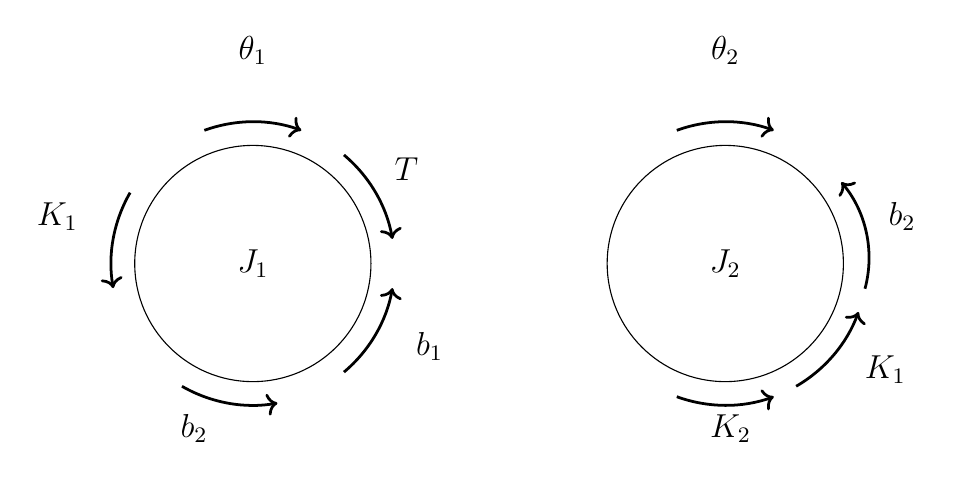
\begin{tikzpicture}[scale=1.5, every node/.style={font=\large}]

    % Circle for J1
    \node[circle, draw, minimum size=3cm] (inertia) at (0,0) {$J_1$};

    % theta1
    \draw[<-, line width=1pt] (70:1.2cm) arc[start angle=70, end angle=110, radius=1.2cm];
    \node at (0,1.8) {$\theta_1$};

    %torque
    \draw[->, line width=1pt] (50:1.2cm) arc[start angle=50, end angle=10, radius=1.2cm];
    \node at (1.3,0.8) {$T$};
    
    % b1 
    \draw[->, line width=1pt] (310:1.2cm) arc[start angle=310, end angle=350, radius=1.2cm];
    \node[anchor=west] at (1.3,-0.7) {$b_1$};

    % b2 (kept bottom-left, adjusted outward)
    \draw[->, line width=1pt] (240:1.2cm) arc[start angle=240, end angle=280, radius=1.2cm];
    \node[anchor=east] at (-0.3,-1.4) {$b_2$};
    
    % K1 (adjusted slightly upward-left)
    \draw[->, line width=1pt] (150:1.2cm) arc[start angle=150, end angle=190, radius=1.2cm];
    \node[anchor=east] at (-1.4,0.4) {$K_1$};


\begin{scope}[shift={(4,0)}]

    % Circle for J2
    \node[circle, draw, minimum size=3cm] (inertia) at (0,0) {$J_2$};

    % theta2
    \draw[<-, line width=1pt] (70:1.2cm) arc[start angle=70, end angle=110, radius=1.2cm];
    \node at (0,1.8) {$\theta_2$};
    
    % b2
    \draw[<-, line width=1pt] (35:1.2cm) arc[start angle=40, end angle=-15, radius=1cm];
    \node[anchor=west] at (1.3,0.4) {$b_2$};
    
    % k1
    \draw[->, line width=1pt] (300:1.2cm) arc[start angle=300, end angle=340, radius=1.2cm];
    \node[anchor=west] at (1.1,-0.9) {$K_1$};

    % k2
    \draw[->, line width=1pt] (250:1.2cm) arc[start angle=250, end angle=290, radius=1.2cm];
    \node[anchor=east] at (0.3,-1.4) {$K_2$};

\end{scope}
\end{tikzpicture}
\end{figure}

Equations of Motion:
\[
T(s) = 2 s^2 \theta_1(s) + 8 \theta_1(s) + 1 \big(\theta_1(s) - \theta_2(s)\big) + 9 \theta_1(s) + 9 \big(\theta_1(s) - \theta_2(s)\big)
\]

Simplify:
\[
T(s) = (2 s^2 + 8 + 9 + 9)\theta_1(s) - (1 + 9)\theta_2(s)
\]
\[
T(s) = (2 s^2 + 26)\theta_1(s) - 10 \theta_2(s)
\]

For inertia $J_2$:
\[
0 = 3 s^2 \theta_2(s) + 1 (\theta_2 - \theta_1) + 9 (\theta_2 - \theta_1) + 7 (\theta_2 - \theta_3)
\]
\[
0 = 3 s^2 \theta_2(s) + 10(\theta_2 - \theta_1) + 7 (\theta_2 - \theta_3)
\]
\[
0 = 3 s^2 \theta_2(s) + 17 \theta_2 - 10 \theta_1 - 7 \theta_3
\]

For inertia $J_3$:
\[
0 = 4 s^2 \theta_3(s) + 2 \theta_3 + 7 (\theta_3 - \theta_2)
\]
\[
0 = 4 s^2 \theta_3(s) + 9 \theta_3 - 7 \theta_2
\]

From $J_3$ equation:
\[
7 \theta_2 = 4 s^2 \theta_3 + 9 \theta_3
\quad 
\]
\[
\quad
\theta_2(s) = \frac{4 s^2 + 9}{7} \theta_3(s)
\]

From $J_2$ equation:
\[
3 s^2 \theta_2 + 17 \theta_2 - 10 \theta_1 - 7 \theta_3 = 0
\quad
\]
\[
\quad
\theta_1(s) = \frac{3 s^2 + 17}{10} \theta_2(s) - \frac{7}{10} \theta_3(s)
\]

Substitute into $J_1$ equation:
\[
T(s) = (2 s^2 + 26)\theta_1(s) - 10 \theta_2(s)
\]

\[
H(s) = \frac{\theta_3(s)}{T(s)} = \frac{7 \cdot 9}{(2 s^2 + 26)\big(3 s^2 + 17 + 7\big)(4 s^2 + 9) - 10^2 (4 s^2 + 9) - 7^2 (2 s^2 + 26)}
\]

\[
(2 s^2 + 27)((3 s^2 + 17)(4 s^2 + 9) - 49) - 100 (4 s^2 + 9) = 24 s^6 + 514 s^4 + 2373 s^2 + 1908
\]

\[
\boxed{
\frac{\theta_3(s)}{T(s)} = \frac{70}{24 s^6 + 514 s^4 + 2373 s^2 + 1908}
}
\]

% Problem 18
\newpage

\noindent\rule{\textwidth}{1pt}
\noindent\textbf{Problem 18} \hfill
\\ Determine the transfer function \(H(s) = \frac{\theta_1(s)}{T(s)}\) for the rotational system shown below.
\begin{figure}[!ht]
\resizebox{1\textwidth}{!}{%
\centering
\begin{tikzpicture}[scale=0.7, transform shape, font=\large]

    % ground and walls
    \draw[pattern=bricks] (6.6,-3) rectangle (8.3,-3.6);
    \draw[pattern=bricks] (-5.8,-1.5) rectangle (-5,2);    
    \draw[pattern=bricks] (16.3,-1.5) rectangle (17.1,1.5);
    
     % fv1
    \pic [scale=1.75] at (-5,0) {damper}; 
    \node at (-2.5,1.2) {8 $N \cdotp m\cdotp s/rad$};

    % fv2
    \pic [scale=1.35] at (3.25,0.5) {damper}; 
    \node at (5,1.5) {4 $N \cdotp m\cdotp s/rad$};
    \draw (7,0.5) -- (7,-0.6); 

    % fv3
    \pic [scale=0.9] at (13.8,0.6) {damper}; 
    \node at (14.8,1.3) {4 $N \cdotp m\cdotp s/rad$};
    
    % fv4
    \pic [scale=1.05, rotate=90] at (7.5,0-3) {damper}; 
    \node at (9,-2.4) {4 $N \cdotp m\cdotp s/rad$};  

    % k1
    \pic [scale=1.85] at (3.25,-0.6) {coil spring};
    \node at (5,-1.2) {$3 N \cdotp m/rad$};

    % k2
    \pic [scale=1.8] at (7,0) {coil spring};
    \node at (8.7,0.8) {$1 N \cdotp m/rad$};

    % k3
    \pic [scale=1.2] at (13.9,-0.4) {coil spring};
    \node at (14.9,-1.3) {$2 N \cdotp m/rad$};

    % j1
    \draw (0,0) ellipse (0.3cm and 1cm);  
    \draw (0,1) -- (3,1);                 
    \draw (0,-1) -- (3,-1);               
    \draw (3,1) arc[start angle=90, end angle=-90, x radius=0.3cm, y radius=1cm]; 
    \node at (1.7,0) {$4kg-m^2$};

    % j2
    \draw (10.6,0) ellipse (0.3cm and 1cm);  
    \draw (10.6,1) -- (13.6,1);                 
    \draw (10.6,-1) -- (13.6,-1);               
    \draw (13.6,1) arc[start angle=90, end angle=-90, x radius=0.3cm, y radius=1cm]; 
    \node at (12.4,0) {$8kg-m^2$};
    
    % t1
    \draw[->, thick, color=cyan] (2,-1.3) arc[start angle=290, end angle=45, x radius=0.5cm, y radius=1.5cm];
    \node at (2,2) {$\theta_1$};
    
     % torque
    \draw[->, thick, color=cyan] (12.5,-1.3) arc[start angle=290, end angle=45, x radius=0.5cm, y radius=1.5cm];
    \node at (12.5,2) {$T$};

\end{tikzpicture}
}%
\end{figure}

\noindent\rule{\textwidth}{1pt}
\vspace{6pt}
\textbf{Given:}
\[
J_1 = 4\ \mathrm{kg\cdot m^2},\quad J_2 = 8\ \mathrm{kg\cdot m^2}
\]
\[
k_1 = 3,\ k_2 = 1,\ k_3 = 2\ \mathrm{N\cdot m/rad}
\]
\[
b_1 = 8,\ b_2 = 4,\ b_3 = 4,\ b_4 = 4\ \mathrm{N\cdot m\cdot s/rad}
\]
\[
T(t) \text{ applied at second rotor}
\]
\[
\theta_1(t),\ \theta_2(t)
\]

\textbf{Required:}
\[
H(s) = \frac{\theta_2(s)}{T(s)}
\]

\textbf{Solution:}

Free Body Diagram

\begin{figure}[!ht]
\centering
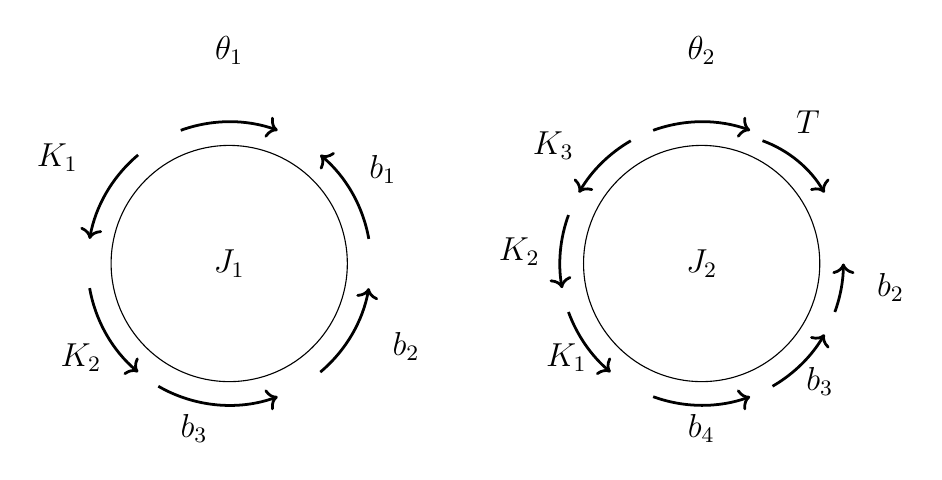
\begin{tikzpicture}[scale=1.5, every node/.style={font=\large}]

    % Circle for J1
    \node[circle, draw, minimum size=3cm] (inertia) at (0,0) {$J_1$};

    % theta1
    \draw[<-, line width=1pt] (70:1.2cm) arc[start angle=70, end angle=110, radius=1.2cm];
    \node at (0,1.8) {$\theta_1$};

    %b1
    \draw[<-, line width=1pt] (50:1.2cm) arc[start angle=50, end angle=10, radius=1.2cm];
    \node at (1.3,0.8) {$b_1$};
    
    % b2
    \draw[->, line width=1pt] (310:1.2cm) arc[start angle=310, end angle=350, radius=1.2cm];
    \node[anchor=west] at (1.3,-0.7) {$b_2$};

    % b3
    \draw[->, line width=1pt] (240:1.2cm) arc[start angle=240, end angle=290, radius=1.2cm];
    \node[anchor=east] at (-0.1,-1.4) {$b_3$};
    
    % K1 
    \draw[->, line width=1pt] (130:1.2cm) arc[start angle=130, end angle=170, radius=1.2cm];
    \node[anchor=east] at (-1.2,0.9) {$K_1$};

    % K2
    \draw[->, line width=1pt] (190:1.2cm) arc[start angle=190, end angle=230, radius=1.2cm];
    \node[anchor=east] at (-1,-0.8) {$K_2$};

\begin{scope}[shift={(4,0)}]

    % Circle for J2
    \node[circle, draw, minimum size=3cm] (inertia) at (0,0) {$J_2$};

    % theta2
    \draw[<-, line width=1pt] (70:1.2cm) arc[start angle=70, end angle=110, radius=1.2cm];
    \node at (0,1.8) {$\theta_2$};
    
    % torque
    \draw[->, line width=1pt] (120:1.2cm) arc[start angle=120, end angle=150, radius=1.2cm];
    \node at (0.9,1.2) {$T$};

    % b2
    \draw[->, line width=1pt] (160:1.2cm) arc[start angle=160, end angle=190, radius=1.2cm];
    \node at (1.6,-0.2) {$b_2$};

    % b3
    \draw[->, line width=1pt] (200:1.2cm) arc[start angle=200, end angle=230, radius=1.2cm];
    \node at (1,-1) {$b_3$};
    
    % b4
    \draw[<-, line width=1pt] (30:1.2cm) arc[start angle=30, end angle=70, radius=1cm];
    \node[anchor=west] at (-0.2,-1.4) {$b_4$};
    
    % k1
    \draw[->, line width=1pt] (300:1.2cm) arc[start angle=300, end angle=330, radius=1.2cm];
    \node[anchor=west] at (-1.4,-0.8) {$K_1$};

    % k2
    \draw[->, line width=1pt] (340:1.2cm) arc[start angle=340, end angle=360, radius=1.2cm];
    \node[anchor=west] at (-1.8,0.1) {$K_2$};

    % k3
    \draw[->, line width=1pt] (250:1.2cm) arc[start angle=250, end angle=290, radius=1.2cm];
    \node[anchor=east] at (-1,1) {$K_3$};

\end{scope}
\end{tikzpicture}
\end{figure}

Inertia 1:
\[
-(K_1 + D_2)(\theta_1 - \theta_m) - D_1 \theta_1 = J_1 s^2 \theta_1
\]
\[
-(3 + 4)(\theta_1 - \theta_m) - 8 \theta_1 = 4s^2 \theta_1
\]
\[
-7(\theta_1 - \theta_m) - 8\theta_1 = 4s^2 \theta_1
\]
\[
-7\theta_1 + 7\theta_m - 8\theta_1 = 4s^2 \theta_1
\]
\[
7\theta_m = (4s^2 + 15)\theta_1 \tag{1}
\]

Inertia 2:
\[
T(s) - (K_2 + D_4)(\theta_2 - \theta_m) - (K_3 + D_3)\theta_2 = J_2 s^2 \theta_2
\]
\[
T(s) - (1 + 4)(\theta_2 - \theta_m) - (2 + 4)\theta_2 = 8s^2 \theta_2
\]
\[
T(s) - 5(\theta_2 - \theta_m) - 6\theta_2 = 8s^2 \theta_2
\]
\[
T(s) - 5\theta_2 + 5\theta_m - 6\theta_2 = 8s^2 \theta_2
\]
\[
T(s) + 5\theta_m = (8s^2 + 11)\theta_2 \tag{2}
\]

From (1):
\[
\theta_m = \frac{(4s^2 + 15)}{7} \theta_1 \tag{3}
\]

Substitute (3) into (2):
\[
T(s) + 5\left( \frac{(4s^2 + 15)}{7} \theta_1 \right) = (8s^2 + 11)\theta_2
\]
\[
T(s) + \frac{20s^2 + 75}{7} \theta_1 = (8s^2 + 11)\theta_2
\]
\[
\theta_2 = \frac{T(s)}{8s^2 + 11} + \frac{20s^2 + 75}{7(8s^2 + 11)} \theta_1 \tag{4}
\]
\[
\theta_1 = \frac{7\theta_m}{4s^2 + 15}
\]
\[
\theta_1 = \frac{7}{4s^2 + 15} \cdot \theta_m
\]

From (2) and (3), substitute \( \theta_m \) and solve for \( \theta_1/T(s) \):
\[
\theta_1 = \frac{7}{4s^2 + 15} \cdot \left( \frac{(8s^2 + 11)\theta_2 - T(s)}{5} \right)
\]

Substitute \( \theta_2 \) from (4):
\[
\theta_1 = \frac{7}{5(4s^2 + 15)} \left[ (8s^2 + 11)\left( \frac{T(s)}{8s^2 + 11} + \frac{20s^2 + 75}{7(8s^2 + 11)} \theta_1 \right) - T(s) \right]
\]

Simplify:
\[
\theta_1 = \frac{7}{5(4s^2 + 15)} \left[ T(s) + \frac{20s^2 + 75}{7} \theta_1 - T(s) \right]
\]
\[
\theta_1 = \frac{7}{5(4s^2 + 15)} \cdot \frac{20s^2 + 75}{7} \theta_1
\]
\[
\theta_1 = \frac{20s^2 + 75}{5(4s^2 + 15)} \theta_1
\]

Divide both sides:
\[
1 = \frac{20s^2 + 75}{5(4s^2 + 15)}
\]
\[
\frac{\theta_1(s)}{T(s)} = \frac{5(4s^2 + 15)}{20s^2 + 75}
\]
\[
\frac{\theta_1(s)}{T(s)}= \frac{20s^2 + 75}{20s^2 + 75}
\]
\[
\frac{\theta_1(s)}{T(s)}= 1
\]

\[
\theta_2 = \frac{T(s)}{8s^2 + 11} + \frac{20s^2 + 75}{7(8s^2 + 11)} \theta_1
\]
\[
\theta_m = \frac{(4s^2 + 15)}{7} \theta_1
\]
\[
T(s) = (8s^2 + 11)\theta_2 - 5\theta_m
\]
\[
T(s)= (8s^2 + 11)\left( \frac{T(s)}{8s^2 + 11} + \frac{20s^2 + 75}{7(8s^2 + 11)} \theta_1 \right) - 5 \cdot \frac{(4s^2 + 15)}{7} \theta_1
\]

Simplify:
\[
T(s) = T(s) + \left( \frac{20s^2 + 75}{7} - \frac{20s^2 + 75}{7} \right) \theta_1
\]
\[
\boxed{
\frac{\theta_1(s)}{T(s)} = \frac{7(8s^2 + 11)}{(20s^2 + 75)(4s^2 + 15)}
}
\]


% Problem 19
\newpage

\noindent\rule{\textwidth}{1pt}
\noindent\textbf{Problem 19} \hfill
\\ Determine the transfer function \(H(s) = \frac{\theta_2(s)}{T(s)}\) for the rotational system shown below.
\begin{figure}[!ht]
\resizebox{1\textwidth}{!}{%
\centering
\begin{tikzpicture}[scale=0.8, transform shape, font=\large]

    % ground and walls
    \draw[pattern=bricks] (3,-3) rectangle (5.1,-3.6);
    \draw[pattern=bricks] (-2.3,-1.5) rectangle (-1.5,1.5);
    \draw[pattern=bricks] (16.3,-1.5) rectangle (17.1,1.5);

    % j1
    \draw (0,0) ellipse (0.3cm and 1cm);  
    \draw (0,1) -- (3,1);                 
    \draw (0,-1) -- (3,-1);               
    \draw (3,1) arc[start angle=90, end angle=-90, x radius=0.3cm, y radius=1cm]; 
    \node at (1.7,0) {$4kg-m^2$};

     % j2
    \draw (10.6,0) ellipse (0.3cm and 1cm);  
    \draw (10.6,1) -- (13.6,1);                 
    \draw (10.6,-1) -- (13.6,-1);               
    \draw (13.6,1) arc[start angle=90, end angle=-90, x radius=0.3cm, y radius=1cm]; 
    \node at (12.4,0) {$8kg-m^2$};

    % fv1
    \pic [scale=1.07, rotate=90] at (4,-3.03) {damper}; 
    \node at (2.6,-2.5) {1 $N \cdotp m\cdotp s/rad$};                
    
    % fv2
    \pic [scale=0.96] at (4.6,0.5) {damper}; 
    \node at (5.8,1.2) {2 $N \cdotp m\cdotp s/rad$};

    % fv3
    \pic [scale=0.9] at (13.8,0.6) {damper}; 
    \node at (14.8,1.4) {4 $N \cdotp m\cdotp s/rad$};
    
    % k1
    \pic [scale=1.35] at (4.6,-0.6) {coil spring};
    \node at (5.8,-1.2) {$1 N \cdotp m/rad$}; 

    % k2
    \pic [scale=1.6] at (7.3,0) {coil spring};
    \node at (8.8,0.7) {$1 N \cdotp m/rad$};

    % k3
    \pic [scale=1.2] at (13.9,-0.5) {coil spring};
    \node at (15,-1.2) {$2 N \cdotp m/rad$};
    
    % t2
    \draw[->, thick, color=cyan] (12.5,-1.3) arc[start angle=290, end angle=45, x radius=0.5cm, y radius=1.5cm];
    \node at (12.5,2) {$\theta_2$};

    % torque
    \draw[->, thick, color=cyan] (2,-1.3) arc[start angle=290, end angle=45, x radius=0.5cm, y radius=1.5cm];
    \node at (2,2) {$T$};

    % lines
    \draw (-1.5,0) -- (0,0);   
    \draw (3.3,0) -- (4.6,0);   
    \draw (4.6,0.5) -- (4.6,-0.6); 
    \draw (3.3,0) -- (4.6,0);   
    \draw (7.3,0.5) -- (7.3,-0.6); 

\end{tikzpicture}
}%
\end{figure}

\noindent\rule{\textwidth}{1pt}
\vspace{1em}
\textbf{Given:}
\[
J_1 = 4\ \mathrm{kg\cdot m^2},\quad J_2 = 8\ \mathrm{kg\cdot m^2}
\]
\[
k_1 = 1,\ k_2 = 1,\ k_3 = 2\ \mathrm{N\cdot m/rad}
\]
\[
b_1 = 1,\ b_2 = 2,\ b_3 = 4\ \mathrm{N\cdot m\cdot s/rad}
\]
\[
T(t) \text{ applied at first rotor}
\]
\[
\theta_1(t),\ \theta_2(t)
\]
\textbf{Required:}
\[
H(s) = \frac{\theta_2(s)}{T(s)}
\]

\textbf{Solution:}

Free Body Diagram

\begin{figure}[!ht]
\centering
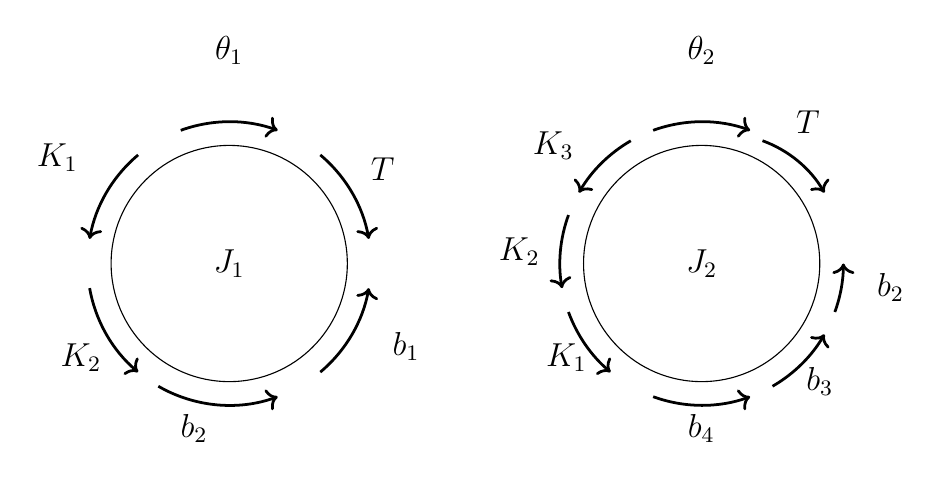
\begin{tikzpicture}[scale=1.5, every node/.style={font=\large}]

    % Circle for J1
    \node[circle, draw, minimum size=3cm] (inertia) at (0,0) {$J_1$};

    % theta1
    \draw[<-, line width=1pt] (70:1.2cm) arc[start angle=70, end angle=110, radius=1.2cm];
    \node at (0,1.8) {$\theta_1$};

    %toqrue
    \draw[->, line width=1pt] (50:1.2cm) arc[start angle=50, end angle=10, radius=1.2cm];
    \node at (1.3,0.8) {$T$};
    
    % b1
    \draw[->, line width=1pt] (310:1.2cm) arc[start angle=310, end angle=350, radius=1.2cm];
    \node[anchor=west] at (1.3,-0.7) {$b_1$};

    % b2
    \draw[->, line width=1pt] (240:1.2cm) arc[start angle=240, end angle=290, radius=1.2cm];
    \node[anchor=east] at (-0.1,-1.4) {$b_2$};
    
    % K1 
    \draw[->, line width=1pt] (130:1.2cm) arc[start angle=130, end angle=170, radius=1.2cm];
    \node[anchor=east] at (-1.2,0.9) {$K_1$};

    % K2
    \draw[->, line width=1pt] (190:1.2cm) arc[start angle=190, end angle=230, radius=1.2cm];
    \node[anchor=east] at (-1,-0.8) {$K_2$};

\begin{scope}[shift={(4,0)}]

    % Circle for J2
    \node[circle, draw, minimum size=3cm] (inertia) at (0,0) {$J_2$};

    % theta2
    \draw[<-, line width=1pt] (70:1.2cm) arc[start angle=70, end angle=110, radius=1.2cm];
    \node at (0,1.8) {$\theta_2$};
    
    % torque
    \draw[->, line width=1pt] (120:1.2cm) arc[start angle=120, end angle=150, radius=1.2cm];
    \node at (0.9,1.2) {$T$};

    % b2
    \draw[->, line width=1pt] (160:1.2cm) arc[start angle=160, end angle=190, radius=1.2cm];
    \node at (1.6,-0.2) {$b_2$};

    % b3
    \draw[->, line width=1pt] (200:1.2cm) arc[start angle=200, end angle=230, radius=1.2cm];
    \node at (1,-1) {$b_3$};
    
    % b4
    \draw[<-, line width=1pt] (30:1.2cm) arc[start angle=30, end angle=70, radius=1cm];
    \node[anchor=west] at (-0.2,-1.4) {$b_4$};
    
    % k1
    \draw[->, line width=1pt] (300:1.2cm) arc[start angle=300, end angle=330, radius=1.2cm];
    \node[anchor=west] at (-1.4,-0.8) {$K_1$};

    % k2
    \draw[->, line width=1pt] (340:1.2cm) arc[start angle=340, end angle=360, radius=1.2cm];
    \node[anchor=west] at (-1.8,0.1) {$K_2$};

    % k3
    \draw[->, line width=1pt] (250:1.2cm) arc[start angle=250, end angle=290, radius=1.2cm];
    \node[anchor=east] at (-1,1) {$K_3$};

\end{scope}
\end{tikzpicture}
\end{figure}

Define angular displacements:
\[
\theta_1(s) \text{ for left inertia}, \quad \theta_2(s) \text{ for right inertia}
\]

Equation for Inertia 1:
\[
\begin{gathered}
T(s) - (K_1 + D_1)(\theta_1 - \theta_m) = J_1 s^2 \theta_1 \\
T(s) - 2(\theta_1 - \theta_m) = 4s^2 \theta_1 \\
T(s) - 2\theta_1 + 2\theta_m = 4s^2 \theta_1 \\
T(s) + 2\theta_m = (4s^2 + 2)\theta_1 \quad \text{(1)}
\end{gathered}
\]

Equation for Inertia 2:
\[
\begin{gathered}
-(K_2 + D_2)(\theta_2 - \theta_m) - (K_3 + D_3)\theta_2 = J_2 s^2 \theta_2 \\
-(\theta_2 - \theta_m) - 6\theta_2 = 8s^2 \theta_2 \\
-\theta_2 + \theta_m - 6\theta_2 = 8s^2 \theta_2 \\
\theta_m = (8s^2 + 7)\theta_2 \quad \text{(2)}
\end{gathered}
\]

Substitute (2) into (1):
\[
T(s) + 2(8s^2 + 7)\theta_2 = (4s^2 + 2)\theta_1
\]
\[
T(s) + 16s^2 \theta_2 + 14\theta_2 = (4s^2 + 2)\theta_1
\]
\[
(4s^2 + 2)\theta_1 = T(s) + 16s^2 \theta_2 + 14\theta_2
\]
\[
\theta_1 = \frac{T(s) + 16s^2 \theta_2 + 14\theta_2}{4s^2 + 2}
\]

Substitute into (1) again to isolate \( \theta_2(s)/T(s) \):
\[
T(s) = (4s^2 + 2)\theta_1 - 16s^2 \theta_2 - 14\theta_2
\]
\[
T(s) = \left( T(s) + 16s^2 \theta_2 + 14\theta_2 \right) - 16s^2 \theta_2 - 14\theta_2
\]
\[
T(s) = T(s)
\]

Isolate \( \theta_2(s) \) from:
\[
T(s) = (4s^2 + 2)\theta_1 - (16s^2 + 14)\theta_2
\]
\[
\theta_2 = \frac{(4s^2 + 2)\theta_1 - T(s)}{16s^2 + 14}
\]

Substitute \( \theta_1 \) from earlier:
\[
\theta_1 = \frac{T(s) + 16s^2 \theta_2 + 14\theta_2}{4s^2 + 2}
\]

Plug into previous:
\[
\theta_2 = \frac{(4s^2 + 2)\left( \frac{T(s) + 16s^2 \theta_2 + 14\theta_2}{4s^2 + 2} \right) - T(s)}{16s^2 + 14}
\]

\[
\theta_2 = \frac{T(s) + 16s^2 \theta_2 + 14\theta_2 - T(s)}{16s^2 + 14}
\]

\[
\theta_2 = \frac{(16s^2 + 14)\theta_2}{16s^2 + 14}
\]

\[
\boxed{
\frac{\theta_2(s)}{T(s)} = \frac{1}{s^4 + 6.5s^2 + 7}
}
\]

% Problem 20
\newpage

\noindent\rule{\textwidth}{1pt}
\noindent\textbf{Problem 20} \hfill
\\ Determine the transfer function \(H(s) = \frac{\theta_3(s)}{T(s)}\) for the rotational system shown below.

\begin{figure}[!ht]
\resizebox{1\textwidth}{!}{%
\centering
\begin{tikzpicture}[scale=0.7, transform shape, font=\large]

    % walls
    \draw[pattern=bricks] (-3.8,-1.5) rectangle (-3,1.5);
    \draw[pattern=bricks] (16.3,-1.5) rectangle (17.1,1.5);

    % fv1
    \pic [scale=1.05] at (-3,0) {damper}; 
    \node at (-1.6,0.9) {2 $N \cdotp m\cdotp s/rad$};

    % fv2
    \pic [scale=0.85] at (3.2,0.5) {damper};
    \node at (4.2,1.4) {1 $N \cdotp m\cdotp s/rad$};

    % fv3
    \pic [scale=0.85] at (13.9,0.5) {damper};  
    \node at (14.7,1.55) {4 $N \cdotp m\cdotp s/rad$};

    % k1
    \draw (3.25,-0.5) -- (3.8,-0.5);
    \draw[decorate,decoration={coil,aspect=0.5,segment length=1mm,amplitude=1mm}] 
        (3.8,-0.5) -- (4.8,-0.5);
    \draw (4.8,-0.5) -- (5.5,-0.5);
    \node at (4.2,-1.2) {$2 \, N \cdotp m/\text{rad}$};
    
    % k2
    \draw (8.85,0) -- (9.2,0);
    \draw[decorate,decoration={coil,aspect=0.5,segment length=1mm,amplitude=1mm}] 
        (9.2,0) -- (10.2,0);
    \draw (10.2,0) -- (10.5,0);
    \node at (9.9,-1.4) {$8 \, N \cdotp m/\text{rad}$};
    
    % k3
    \draw (13.85,-0.5) -- (14.5,-0.5);
    \draw[decorate,decoration={coil,aspect=0.5,segment length=1mm,amplitude=1mm}] 
        (14.5,-0.5) -- (15.5,-0.5);
    \draw (15.5,-0.5) -- (16.3,-0.5);
    \node at (14.9,-1.2) {$8 \, N \cdotp m/\text{rad}$};
    
    % j1
    \draw (0,0) ellipse (0.3cm and 1cm);  
    \draw (0,1) -- (3,1);                 
    \draw (0,-1) -- (3,-1);               
    \draw (3,1) arc[start angle=90, end angle=-90, x radius=0.3cm, y radius=1cm]; 
    \node at (1.7,0) {$5kg-m^2$};
    
    % j2
    \draw (5.6,0) ellipse (0.3cm and 1cm);  
    \draw (5.6,1) -- (8.6,1);                 
    \draw (5.6,-1) -- (8.6,-1);               
    \draw (8.6,1) arc[start angle=90, end angle=-90, x radius=0.3cm, y radius=1cm]; 
    \node at (7.3,0) {$4kg-m^2$};

    % j3
    \draw (10.6,0) ellipse (0.3cm and 1cm);  
    \draw (10.6,1) -- (13.6,1);                 
    \draw (10.6,-1) -- (13.6,-1);               
    \draw (13.6,1) arc[start angle=90, end angle=-90, x radius=0.3cm, y radius=1cm]; 
    \node at (12.1,0) {$2kg-m^2$};
    
    % t1
    \draw[->, thick, color=cyan] (2,-1.3) arc[start angle=290, end angle=45, x radius=0.5cm, y radius=1.5cm];
    \node at (2,2) {$\theta_1$};
    
    % t2
    \draw[->, thick, color=cyan] (7,-1.3) arc[start angle=290, end angle=45, x radius=0.5cm, y radius=1.5cm];
    \node at (7,2) {$\theta_2$};

    % t3
    \draw[->, thick, color=cyan] (12.5,-1.3) arc[start angle=290, end angle=45, x radius=0.5cm, y radius=1.5cm];
    \node at (12.5,2) {$\theta_3$};
    
    % torque
    \draw[->, thick, color=cyan] (8,-1.3) arc[start angle=290, end angle=45, x radius=0.5cm, y radius=1.5cm];
    \node at (8,2) {$T$};
    
\end{tikzpicture}
}%
\end{figure}

\noindent\rule{\textwidth}{1pt}

\textbf{Given:}
\[
J_1 = 5\ \mathrm{kg\cdot m^2},\quad J_2 = 4\ \mathrm{kg\cdot m^2},\quad J_3 = 2\ \mathrm{kg\cdot m^2}
\]
\[
k_1 = 2\ \mathrm{N\cdot m/rad},\quad k_2 = 8\ \mathrm{N\cdot m/rad},\quad k_3 = 8\ \mathrm{N\cdot m/rad}
\]
\[
b_1 = 2\ \mathrm{N\cdot m\cdot s/rad},\quad b_2 = 1\ \mathrm{N\cdot m\cdot s/rad},\quad b_3 = 4\ \mathrm{N\cdot m\cdot s/rad}
\]
\[
T(t) \text{ applied at second rotor}
\]
\[
\theta_1(t),\ \theta_2(t),\ \theta_3(t)
\]

\textbf{Required:}
\[
H(s) = \frac{\theta_3(s)}{T(s)}
\]

\textbf{Solution:}

Free Body Diagram

\begin{figure}[!ht]
\centering
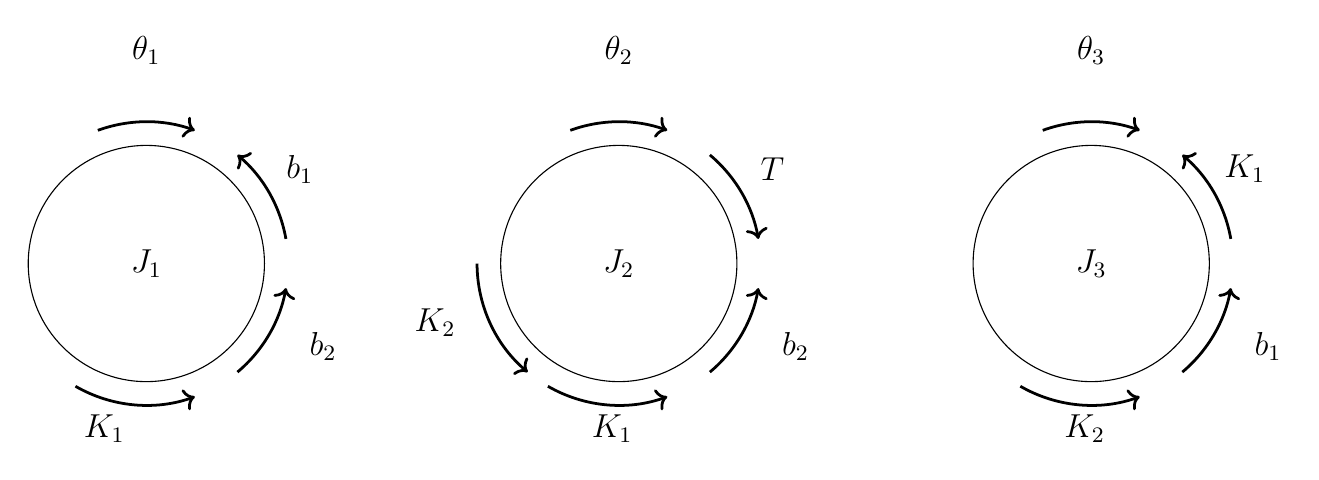
\begin{tikzpicture}[scale=1.5, every node/.style={font=\large}]

    % Circle for J1
    \node[circle, draw, minimum size=3cm] (inertia) at (0,0) {$J_1$};

    % theta1
    \draw[<-, line width=1pt] (70:1.2cm) arc[start angle=70, end angle=110, radius=1.2cm];
    \node at (0,1.8) {$\theta_1$};

    % b1
    \draw[<-, line width=1pt] (50:1.2cm) arc[start angle=50, end angle=10, radius=1.2cm];
    \node at (1.3,0.8) {$b_1$};
    
    % b2
    \draw[->, line width=1pt] (310:1.2cm) arc[start angle=310, end angle=350, radius=1.2cm];
    \node[anchor=west] at (1.3,-0.7) {$b_2$};

    % k1
    \draw[->, line width=1pt] (240:1.2cm) arc[start angle=240, end angle=290, radius=1.2cm];
    \node[anchor=east] at (-0.1,-1.4) {$K_1$};

\begin{scope}[shift={(4,0)}]

    % Circle for J2
    \node[circle, draw, minimum size=3cm] (inertia) at (0,0) {$J_2$};

    % theta2
    \draw[<-, line width=1pt] (70:1.2cm) arc[start angle=70, end angle=110, radius=1.2cm];
    \node at (0,1.8) {$\theta_2$};

    % torque
    \draw[->, line width=1pt] (50:1.2cm) arc[start angle=50, end angle=10, radius=1.2cm];
    \node at (1.3,0.8) {$T$};
    
    % b2
    \draw[->, line width=1pt] (310:1.2cm) arc[start angle=310, end angle=350, radius=1.2cm];
    \node[anchor=west] at (1.3,-0.7) {$b_2$};

    % k1
    \draw[->, line width=1pt] (240:1.2cm) arc[start angle=240, end angle=290, radius=1.2cm];
    \node[anchor=east] at (0.2,-1.4) {$K_1$};

    % k2
    \draw[->, line width=1pt] (180:1.2cm) arc[start angle=180, end angle=230, radius=1.2cm];
    \node[anchor=east] at (-1.3,-0.5) {$K_2$};

\end{scope}
\begin{scope}[shift={(8,0)}]

    % Circle for J3
    \node[circle, draw, minimum size=3cm] (inertia) at (0,0) {$J_3$};

    % theta3
    \draw[<-, line width=1pt] (70:1.2cm) arc[start angle=70, end angle=110, radius=1.2cm];
    \node at (0,1.8) {$\theta_3$};

    % K1
    \draw[<-, line width=1pt] (50:1.2cm) arc[start angle=50, end angle=10, radius=1.2cm];
    \node at (1.3,0.8) {$K_1$};
    
    % b
    \draw[->, line width=1pt] (310:1.2cm) arc[start angle=310, end angle=350, radius=1.2cm];
    \node[anchor=west] at (1.3,-0.7) {$b_1$};

    % k2
    \draw[->, line width=1pt] (240:1.2cm) arc[start angle=240, end angle=290, radius=1.2cm];
    \node[anchor=east] at (0.2,-1.4) {$K_2$};

\end{scope}
\end{tikzpicture}
\end{figure}

For Inertia 1:
\[
J_1 s^2 \theta_1(s) + b_1 \left[\theta_1(s) - 0\right] + b_2 \left[\theta_1(s) - \theta_2(s)\right] + k_1 \left[\theta_1(s) - 0\right] + k_2 \left[\theta_1(s) - \theta_2(s)\right] = 0
\]
\[
( J_1 s^2 + b_1 + b_2 + k_1 + k_2 ) \theta_1(s) - (b_2 + k_2) \theta_2(s) = 0
\]

For Inertia 2:
\[
0 =\ J_2 s^2 \theta_2(s) 
    + (b_2 + k_2)\big[\theta_2(s) - \theta_1(s)\big] 
    + (b_3 + k_3)\big[\theta_2(s) - \theta_3(s)\big]
\]
\[
-(b_2 + k_2)\theta_1(s) 
+ (J_2 s^2 + b_2 + b_3 + k_2 + k_3)\theta_2(s) 
- (b_3 + k_3) \theta_3(s) 
= 0
\]

For Inertia 3:
\[
J_3 s^2 \theta_3(s) + b_3 \left[\theta_3(s) - \theta_2(s)\right] + k_3 \left[\theta_3(s) - \theta_2(s)\right] = T(s)
\]
\[
-(b_3 + k_3)\theta_2(s) + (J_3 s^2 + b_3 + k_3) \theta_3(s) = T(s)
\]

Substitute numerical values:

Inertia 1:
\[
(5 s^2 + 2 + 1 + 2 + 8) \theta_1 - (1 + 8) \theta_2 = 0
\]
\[
(5 s^2 + 13)\theta_1 - 9 \theta_2 = 0
\]

Inertia 2:
\[
-(1+8)\theta_1 + (4 s^2 + 1 + 4 + 8 + 8)\theta_2 - (4+8)\theta_3 = 0
\]
\[
-9 \theta_1 + (4 s^2 + 21)\theta_2 - 12 \theta_3 = 0
\]

Inertia 3:
\[
-(4+8)\theta_2 + (2 s^2 + 4 + 8)\theta_3 = T(s)
\]
\[
-12 \theta_2 + (2 s^2 + 12) \theta_3 = T(s)
\]

Solve the system using determinants (Cramer's Rule):

\[
\begin{bmatrix}
5s^2 + 13 & -9 & 0 \\
-9 & 4s^2 + 21 & -12 \\
0 & -12 & 2s^2 + 12
\end{bmatrix}
\begin{bmatrix}
\theta_1 \\ \theta_2 \\ \theta_3
\end{bmatrix}
=
\begin{bmatrix}
0 \\ 0 \\ T(s)
\end{bmatrix}
\]

Determinant of coefficient matrix:

\[
\Delta = 
\begin{vmatrix}
5s^2 + 13 & -9 & 0 \\
-9 & 4s^2 + 21 & -12 \\
0 & -12 & 2s^2 + 12
\end{vmatrix}
\]

Expand along first row:
\[
\Delta = (5s^2+13)\begin{vmatrix}4s^2+21 & -12 \\ -12 & 2s^2+12\end{vmatrix} - (-9) \begin{vmatrix}-9 & -12 \\ 0 & 2s^2+12 \end{vmatrix}
\]

Compute subdeterminants:
\[
\begin{vmatrix}
4s^2+21 & -12 \\
-12 & 2s^2+12
\end{vmatrix}
= (4s^2+21)(2s^2+12) - (-12)^2  = 8s^4 + 120s^2 + 108
\]

\[
\begin{vmatrix}
-9 & -12 \\
0 & 2s^2+12
\end{vmatrix}
= (-9)(2s^2+12) - (0)(-12) = -18s^2 - 108
\]

\[
\begin{vmatrix}
-9 & -12 \\
0 & 2s^2+12
\end{vmatrix}
= -9(2s^2+12) = -18s^2 - 108
\]

\[
\Delta = (5s^2+13)(8 s^4 + 120 s^2 + 108) + 9(-18 s^2 -108)
\]
\[
\Delta = (5s^2+13)(8 s^4 + 120 s^2 + 108) - 162 s^2 - 972
\]

Multiply:
\[
(5s^2)(8 s^4 + 120 s^2 + 108) = 40 s^6 + 600 s^4 + 540 s^2
\]
\[
13(8 s^4 + 120 s^2 + 108) = 104 s^4 + 1560 s^2 + 1404
\]
\[
(40 s^6 + 704 s^4 + 2100 s^2 + 1404) - (162 s^2 + 972) = 40 s^6 + 704 s^4 + 1938 s^2 + 432
\]

Determinant for \(\theta_3\):

\[
\Delta_3 = 
\begin{vmatrix}
5 s^2 + 13 & -9 & 0 \\
-9 & 4s^2 + 21 & 0 \\
0 & -12 & T(s)
\end{vmatrix}
= T(s) \begin{vmatrix}5s^2 + 13 & -9 \\ -9 & 4s^2 + 21 \end{vmatrix}
\]

\[
\begin{vmatrix}5s^2 + 13 & -9 \\ -9 & 4s^2 + 21 \end{vmatrix} 
= (5s^2 +13)(4s^2+21) - (-9)(-9) 
\]
\[
= 20 s^4 + 105 s^2 + 273 - 81 
\]
\[
= 20 s^4 + 105 s^2 + 192
\]

Transfer function:
\[
H(s) = \frac{\theta_3(s)}{T(s)} = \frac{\Delta_3}{\Delta} = \frac{20 s^4 + 105 s^2 + 192}{40 s^6 + 704 s^4 + 1938 s^2 + 432}
\]

\[
\boxed{H(s) = \frac{20 s^4 + 105 s^2 + 192}{40 s^6 + 704 s^4 + 1938 s^2 + 432}}
\]

% Problem 21
\newpage

\noindent\rule{\textwidth}{1pt}
\noindent\textbf{Problem 21} \hfill
\\ Determine the transfer function \(H(s) = \frac{\theta_2(s)}{T(s)}\) for the rotational system shown below.

\begin{figure}[!ht]
\centering
\resizebox{1\textwidth}{!}{%
\begin{tikzpicture}[scale=1.4, transform shape, font=\large]

    % ground and walls
    \draw[pattern=bricks] (1.6,-3.4) rectangle (5.3,-4.0); 
    \draw[pattern=bricks] (-2.0,-1.5) rectangle (-2.8,1.5);
    \draw[pattern=bricks] (13.6,-1.5) rectangle (14.4,1.5);

    % fv1
    \pic [scale=1] at (-2,0) {damper};            
    \node at (-0.7,0.9) {$3\,\mathrm{N \cdotp m\cdotp s/rad}$};

    % fv2
    \pic [scale=1.2, rotate=90] at (4.5,-3.4) {damper};              
    \node at (5.9,-2.7) {$2\,\mathrm{N \cdotp m\cdotp s/rad}$}; 

    % fv3
    \pic [scale=1.05] at (10.8,0) {damper};                 
    \node at (12.0,0.8) {$6\,\mathrm{N \cdotp m\cdotp s/rad}$};

    % k1
    \pic [scale=1.2, rotate=90] at (2.5,-3.4) {coil spring};
    \node at (1,-2.4) {$4\,\mathrm{N \cdotp m/rad}$};

    % k2
    \pic [scale=1.7] at (4.1,0) {coil spring};
    \node at (5.7,0.5) {$5\,\mathrm{N \cdotp m/rad}$};
    
    % j1
    \draw (0.8,0) ellipse (0.3cm and 1cm);  
    \draw (0.8,1) -- (3.8,1);                 
    \draw (0.8,-1) -- (3.8,-1);               
    \draw (3.8,1) arc[start angle=90, end angle=-90, x radius=0.3cm, y radius=1cm]; 
    \node at (2.5,0) {$6kg-m^2$};

    % j2
    \draw (7.5,0) ellipse (0.3cm and 1cm);  
    \draw (7.5,1) -- (10.5,1);                 
    \draw (7.5,-1) -- (10.5,-1);               
    \draw (10.5,1) arc[start angle=90, end angle=-90, x radius=0.3cm, y radius=1cm]; 
    \node at (9.2,0) {$5kg-m^2$};

    % t1
    \draw[->, thick, color=cyan] (2.5,-1.3) arc[start angle=290, end angle=45, x radius=0.5cm, y radius=1.5cm];
    \node at (2.5,2) {$\theta_1$};
    
    % t2
    \draw[->, thick, color=cyan] (9.5,-1.3) arc[start angle=290, end angle=45, x radius=0.5cm, y radius=1.5cm];
    \node at (9.5,2) {$\theta_2$};

    % torque
    \draw[->, thick, color=cyan] (8.7,-1.3) arc[start angle=290, end angle=45, x radius=0.5cm, y radius=1.5cm];
    \node at (8.7,2) {$T$};
    
\end{tikzpicture}
}%
\end{figure}


\noindent\rule{\textwidth}{1pt}
\textbf{Given:}
\[
J_1 = 6\ \mathrm{kg\cdot m^2},\quad J_2 = 5\ \mathrm{kg\cdot m^2}
\]
\[
k_1 = 4,\ k_2 = 5\ \mathrm{N\cdot m/rad}
\]
\[
 b_1 = 3,\ b_2 = 2,\ b_3 = 6\ \mathrm{N\cdot m\cdot s/rad}
\]
\[
T(t) \text{ applied at second rotor}
\]
\[
\theta_1(t),\ \theta_2(t)
\]

\textbf{Required:}
\[
H(s) = \frac{\theta_2(s)}{T(s)}
\]


\textbf{Solution: }

Free Body Diagram

\begin{figure}[!ht]
\centering
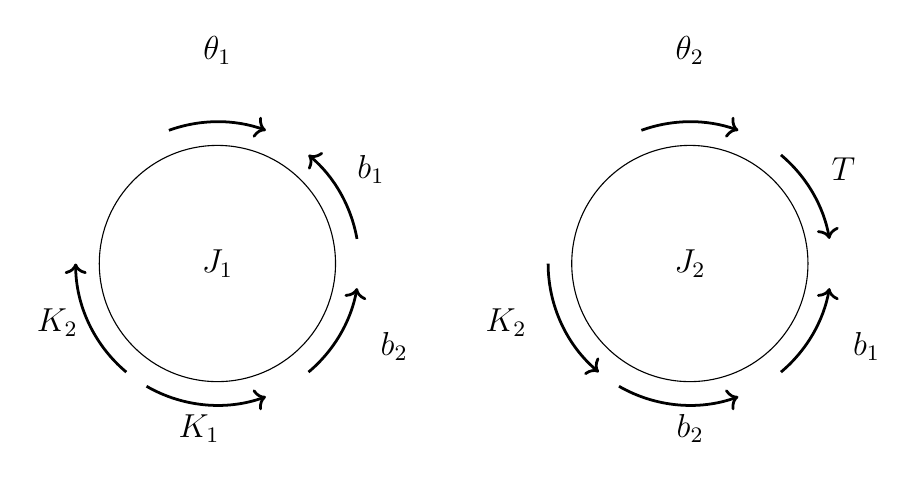
\begin{tikzpicture}[scale=1.5, every node/.style={font=\large}]

    % Circle for J1
    \node[circle, draw, minimum size=3cm] (inertia) at (0,0) {$J_1$};

    % theta1
    \draw[<-, line width=1pt] (70:1.2cm) arc[start angle=70, end angle=110, radius=1.2cm];
    \node at (0,1.8) {$\theta_1$};

    % b1
    \draw[<-, line width=1pt] (50:1.2cm) arc[start angle=50, end angle=10, radius=1.2cm];
    \node at (1.3,0.8) {$b_1$};
    
    % b2
    \draw[->, line width=1pt] (310:1.2cm) arc[start angle=310, end angle=350, radius=1.2cm];
    \node[anchor=west] at (1.3,-0.7) {$b_2$};

    % k1
    \draw[->, line width=1pt] (240:1.2cm) arc[start angle=240, end angle=290, radius=1.2cm];
    \node[anchor=east] at (0.1,-1.4) {$K_1$};

    % k2
    \draw[->, line width=1pt] (230:1.2cm) arc[start angle=230, end angle=180, radius=1.2cm];
    \node[anchor=east] at (-1.1,-0.5) {$K_2$};

\begin{scope}[shift={(4,0)}]

    % Circle for J2
    \node[circle, draw, minimum size=3cm] (inertia) at (0,0) {$J_2$};

    % theta2
    \draw[<-, line width=1pt] (70:1.2cm) arc[start angle=70, end angle=110, radius=1.2cm];
    \node at (0,1.8) {$\theta_2$};

    % torque
    \draw[->, line width=1pt] (50:1.2cm) arc[start angle=50, end angle=10, radius=1.2cm];
    \node at (1.3,0.8) {$T$};
    
    % b1
    \draw[->, line width=1pt] (310:1.2cm) arc[start angle=310, end angle=350, radius=1.2cm];
    \node[anchor=west] at (1.3,-0.7) {$b_1$};

    % b2
    \draw[->, line width=1pt] (240:1.2cm) arc[start angle=240, end angle=290, radius=1.2cm];
    \node[anchor=east] at (0.2,-1.4) {$b_2$};

    % k2
    \draw[->, line width=1pt] (180:1.2cm) arc[start angle=180, end angle=230, radius=1.2cm];
    \node[anchor=east] at (-1.3,-0.5) {$K_2$};

\end{scope}
\end{tikzpicture}
\end{figure}

Torque balance on Inertia 1:
\[
T(s) - D_A \theta_1 - K_1 \theta_1 - D_B (\theta_1 - \theta_2) - K_2 (\theta_1 - \theta_2) = J_1 s^2 \theta_1
\]
\[
T(s) - (D_A + K_1)\theta_1 - (D_B + K_2)(\theta_1 - \theta_2) = J_1 s^2 \theta_1
\]
\[
T(s) - (3 + 4)\theta_1 - (2 + 5)(\theta_1 - \theta_2) = 6s^2 \theta_1
\]
\[
T(s) - 7\theta_1 - 7(\theta_1 - \theta_2) = 6s^2 \theta_1
\]
\[
T(s) - 14\theta_1 + 7\theta_2 = 6s^2 \theta_1
\]
\[
T(s) + 7\theta_2 = (6s^2 + 14)\theta_1 \quad \text{(1)}
\]

Torque balance on Inertia 2:
\[
- D_C \theta_2 - (D_B + K_2)(\theta_2 - \theta_1) = J_2 s^2 \theta_2
\]
\[
- 6\theta_2 - 7(\theta_2 - \theta_1) = 5s^2 \theta_2
\]
\[
- 6\theta_2 - 7\theta_2 + 7\theta_1 = 5s^2 \theta_2
\]
\[
-13\theta_2 + 7\theta_1 = 5s^2 \theta_2
\]
\[
7\theta_1 = (5s^2 + 13)\theta_2 \quad \text{(2)}
\]

Substitute (2) into (1):
\[
T(s) + 7\theta_2 = (6s^2 + 14)\left( \frac{(5s^2 + 13)\theta_2}{7} \right)
\]
\[
T(s) + 7\theta_2 = \frac{(6s^2 + 14)(5s^2 + 13)}{7} \theta_2
\]
\[
T(s) = \left( \frac{(6s^2 + 14)(5s^2 + 13)}{7} - 7 \right) \theta_2
\]
\[
\frac{\theta_2(s)}{T(s)} = \frac{1}{\frac{(6s^2 + 14)(5s^2 + 13)}{7} - 7}
\]
\[
\frac{\theta_2(s)}{T(s)} = \frac{1}{\frac{30s^4 + 182s^2 + 182}{7} - 7}
\]
\[
\frac{\theta_2(s)}{T(s)} = \frac{1}{\frac{30s^4 + 182s^2 + 182 - 49}{7}}
\]
\[
\frac{\theta_2(s)}{T(s)} = \frac{1}{\frac{30s^4 + 182s^2 + 133}{7}}
\]
\[
\frac{\theta_2(s)}{T(s)} = \frac{7}{30s^4 + 182s^2 + 133}
\]

\[
\boxed{\frac{\theta_2(s)}{T(s)} = \frac{7}{30s^4 + 182s^2 + 133}}
\]

% Problem 22
\newpage

\noindent\rule{\textwidth}{1pt}
\noindent\textbf{Problem 22} \hfill
\\ Determine the transfer function \(H(s) = \frac{\theta_o(s)}{T(s)}\) for the rotational system shown below.

\begin{figure}[!ht]
\centering
\resizebox{1\textwidth}{!}{%
\begin{tikzpicture}[scale=1.4, transform shape, font=\large]

    % ground and walls
    \draw[pattern=bricks] (0.2,-3.2) rectangle (1.7,-3.7);
    \draw[pattern=bricks] (8.5,-3.2) rectangle (9.9,-3.7); 
    \draw[pattern=bricks] (-5.5,-1.5) rectangle (-4.7,2);
    \draw[pattern=bricks] (14.5,-1.5) rectangle (15.3,2);

    % j1
    \draw (-1,0) ellipse (0.5cm and 1cm);  
    \draw (-1,1) -- (3,1);                 
    \draw (-1,-1) -- (3,-1);               
    \draw (3,1) arc[start angle=90, end angle=-90, x radius=0.5cm, y radius=1cm]; 
    \node at (1.2,0) {$4\,\mathrm{kg\cdot m^2}$};

    % j2
    \draw (7,0) ellipse (0.5cm and 1cm);  
    \draw (7,1) -- (11,1);                 
    \draw (7,-1) -- (11,-1);               
    \draw (11,1) arc[start angle=90, end angle=-90, x radius=0.5cm, y radius=1cm]; 
    \node at (9.2,0) {$6\,\mathrm{kg\cdot m^2}$};

    % fv1
    \pic [scale=1.25] at (-4.75,0) {damper}; 
    \node at (-3,1) {$5\,\mathrm{N \cdotp m\cdotp s/rad}$};

    % fv2
    \pic [scale=0.8, rotate=90] at (0.9,-3.2) {damper};                
    \node at (2.5,-2.3) {$2\,\mathrm{N \cdotp m\cdotp s/rad}$};

    % fv3
    \pic [scale=1.1] at (11.5,0) {damper}; 
    \node at (12.8,1) {$4\,\mathrm{N \cdotp m\cdotp s/rad}$};

    % k1
    \pic [scale=1.7] at (3.5,0) {coil spring};
    \node at (5,0.8) {$10\,\mathrm{N \cdotp m/rad}$};

    % k2
    \pic [scale=1.1, rotate=90] at (9.2,-3.2) {coil spring};
    \node at (7.6,-2.1) {$7\,\mathrm{N \cdotp m/rad}$};
    
    % t1
    \draw[->, thick, color=cyan] (1.5,-1.3) arc[start angle=290, end angle=45, x radius=0.5cm, y radius=1.5cm];
    \node at (1.5,2) {$\theta_1$};
    
    % t2
    \draw[->, thick, color=cyan] (8.5,-1.3) arc[start angle=290, end angle=45, x radius=0.5cm, y radius=1.5cm];
    \node at (8.5,2) {$\theta_2$};

    % torque
    \draw[->, thick, color=cyan] (9.7,-1.3) arc[start angle=290, end angle=45, x radius=0.5cm, y radius=1.5cm];
    \node at (9.7,2) {$T$};

\end{tikzpicture}
}%
\end{figure}

\noindent\rule{\textwidth}{1pt}
\textbf{Given:}
\[
J_1 = 4\ \mathrm{kg\cdot m^2},\quad J_2 = 6\ \mathrm{kg\cdot m^2}
\]
\[
k_1 = 10,\ k_2 = 7\ \mathrm{N\cdot m/rad}
\]
\[
b_1 = 5,\ b_2 = 2,\ b_3 = 4\ \mathrm{N\cdot m\cdot s/rad}
\]
\[
T(t) \text{ applied at second rotor}
\]
\[
\theta_1(t),\ \theta_2(t)
\]

\textbf{Required:}
\[
H(s) = \frac{\theta_2(s)}{T(s)}
\]

\textbf{Solution:}

Free Body Diagram

\begin{figure}[!ht]
\centering
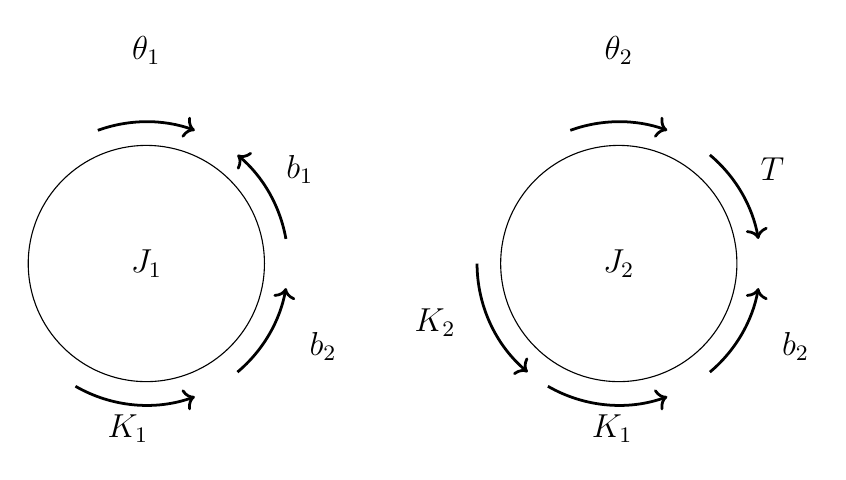
\begin{tikzpicture}[scale=1.5, every node/.style={font=\large}]

    % Circle for J1
    \node[circle, draw, minimum size=3cm] (inertia) at (0,0) {$J_1$};

    % theta1
    \draw[<-, line width=1pt] (70:1.2cm) arc[start angle=70, end angle=110, radius=1.2cm];
    \node at (0,1.8) {$\theta_1$};

    % b1
    \draw[<-, line width=1pt] (50:1.2cm) arc[start angle=50, end angle=10, radius=1.2cm];
    \node at (1.3,0.8) {$b_1$};
    
    % b2
    \draw[->, line width=1pt] (310:1.2cm) arc[start angle=310, end angle=350, radius=1.2cm];
    \node[anchor=west] at (1.3,-0.7) {$b_2$};

    % k1
    \draw[->, line width=1pt] (240:1.2cm) arc[start angle=240, end angle=290, radius=1.2cm];
    \node[anchor=east] at (0.1,-1.4) {$K_1$};
    
\begin{scope}[shift={(4,0)}]

    % Circle for J2
    \node[circle, draw, minimum size=3cm] (inertia) at (0,0) {$J_2$};

    % theta2
    \draw[<-, line width=1pt] (70:1.2cm) arc[start angle=70, end angle=110, radius=1.2cm];
    \node at (0,1.8) {$\theta_2$};

    % torque
    \draw[->, line width=1pt] (50:1.2cm) arc[start angle=50, end angle=10, radius=1.2cm];
    \node at (1.3,0.8) {$T$};
    
    % b2
    \draw[->, line width=1pt] (310:1.2cm) arc[start angle=310, end angle=350, radius=1.2cm];
    \node[anchor=west] at (1.3,-0.7) {$b_2$};

    % k1
    \draw[->, line width=1pt] (240:1.2cm) arc[start angle=240, end angle=290, radius=1.2cm];
    \node[anchor=east] at (0.2,-1.4) {$K_1$};

    % k2
    \draw[->, line width=1pt] (180:1.2cm) arc[start angle=180, end angle=230, radius=1.2cm];
    \node[anchor=east] at (-1.3,-0.5) {$K_2$};

\end{scope}
\end{tikzpicture}
\end{figure}

Torque balance on Inertia 1:
\[
- D_1 \theta_1 - D_2 \theta_1 - K_1 (\theta_1 - \theta_2) = J_1 s^2 \theta_1
\]
\[
- (D_1 + D_2)\theta_1 - K_1(\theta_1 - \theta_2) = J_1 s^2 \theta_1
\]
\[
-7\theta_1 - 10(\theta_1 - \theta_2) = 4s^2 \theta_1
\]
\[
-7\theta_1 - 10\theta_1 + 10\theta_2 = 4s^2 \theta_1
\]
\[
-17\theta_1 + 10\theta_2 = 4s^2 \theta_1
\]
\[
10\theta_2 = (4s^2 + 17)\theta_1 \quad \text{(1)}
\]

Torque balance on Inertia 2:
\[
T(s) - D_3 \theta_2 - K_1 (\theta_2 - \theta_1) - K_2 \theta_2 = J_2 s^2 \theta_2
\]
\[
T(s) - 4\theta_2 - 10(\theta_2 - \theta_1) - 7\theta_2 = 6s^2 \theta_2
\]
\[
T(s) - 4\theta_2 - 10\theta_2 + 10\theta_1 - 7\theta_2 = 6s^2 \theta_2
\]
\[
T(s) + 10\theta_1 - 21\theta_2 = 6s^2 \theta_2
\]
\[
T(s) + 10\theta_1 = (6s^2 + 21)\theta_2 \quad \text{(2)}
\]

Substitute (1) into (2):
\[
T(s) + 10\left( \frac{10\theta_2}{4s^2 + 17} \right) = (6s^2 + 21)\theta_2
\]
\[
T(s) + \frac{100\theta_2}{4s^2 + 17} = (6s^2 + 21)\theta_2
\]
\[
T(s) = \left( 6s^2 + 21 - \frac{100}{4s^2 + 17} \right)\theta_2
\]

\[
\frac{\theta_2(s)}{T(s)} = \frac{1}{6s^2 + 21 - \frac{100}{4s^2 + 17}}
\]

\[
\frac{\theta_2(s)}{T(s)} = \frac{1}{\frac{(6s^2 + 21)(4s^2 + 17) - 100}{4s^2 + 17}}
\]

\[
\frac{\theta_2(s)}{T(s)} = \frac{4s^2 + 17}{(6s^2 + 21)(4s^2 + 17) - 100}
\]

\[
\frac{\theta_2(s)}{T(s)} = \frac{4s^2 + 17}{24s^4 + 102s^2 + 126s^2 + 357 - 100}
\]

\[
\frac{\theta_2(s)}{T(s)} = \frac{4s^2 + 17}{24s^4 + 228s^2 + 257}
\]

\[
\frac{\theta_2(s)}{T(s)} = \frac{4s^2 + 17}{24s^4 + 228s^2 + 257}
\]

\[
\boxed{\frac{\theta_2(s)}{T(s)} = \frac{4s^2 + 17}{24s^4 + 228s^2 + 257}}
\]

% Problem 23
\newpage

\noindent\rule{\textwidth}{1pt}
\noindent\textbf{Problem 23} \hfill
\\ Determine the transfer function \(H(s) = \frac{\theta_3(s)}{T(s)}\) for the rotational system shown below.

\begin{figure}[!ht]
\centering
\resizebox{1\textwidth}{!}{%
\begin{tikzpicture}[scale=1.4, transform shape, font=\medium]

    % walls
    \draw[pattern=bricks] (-4.8,-1.5) rectangle (-4,1.5);
    \draw[pattern=bricks] (14.3,-1.5) rectangle (15.1,1.5);

    % fv1
    \pic [scale=0.7] at (-4,0) {damper}; 
    \node at (-2.7,1.4) {$3\,\mathrm{N \cdotp m\cdotp s/rad}$}; % label above

    % fv2
    \pic [scale=0.8] at (1.3,0.4) {damper};             
    \node at (2.2,1.4) {2 $N \cdotp m\cdotp s/rad$};

    % fv3
    \pic [scale=0.85] at (11.9,0) {damper};                 
    \node at (12.7,1.3) {5 $N \cdotp m\cdotp s/rad$};
    
    % j1
    \draw (-2,0) ellipse (0.3cm and 1cm);  
    \draw (-2,1) -- (1,1);                 
    \draw (-2,-1) -- (1,-1);               
    \draw (1,1) arc[start angle=90, end angle=-90, x radius=0.3cm, y radius=1cm]; 
    \node at (-0.4,0) {$6kg-m^2$};

     % j2
    \draw (3.5,0) ellipse (0.3cm and 1cm);  
    \draw (3.5,1) -- (6.5,1);                 
    \draw (3.5,-1) -- (6.5,-1);               
    \draw (6.5,1) arc[start angle=90, end angle=-90, x radius=0.3cm, y radius=1cm]; 
    \node at (5,0) {$3kg-m^2$};

    % j3
    \draw (8.6,0) ellipse (0.3cm and 1cm);  
    \draw (8.6,1) -- (11.6,1);                 
    \draw (8.6,-1) -- (11.6,-1);               
    \draw (11.6,1) arc[start angle=90, end angle=-90, x radius=0.3cm, y radius=1cm]; 
    \node at (10.1,0) {$1.5kg-m^2$};  

    % k1
    \pic [scale=1.1] at (1.3,-0.4) {coil spring};
    \node at (2.2,-1) {$4 N \cdotp m/rad$};

    % k2
    \pic [scale=0.9] at (6.8,0) {coil spring};
    \node at (7.7,-1.5) {$10 N \cdotp m/rad$};

    % torque
    \draw[->, thick, color=cyan] (0,-1.3) arc[start angle=290, end angle=45, x radius=0.5cm, y radius=1.5cm];
    \node at (0,2) {$T$};

    %t2
    \draw[->, thick, color=cyan] (5.2,-1.3) arc[start angle=290, end angle=45, x radius=0.5cm, y radius=1.5cm];
    \node at (5.2,2) {$\theta_2$};
    
    % t3
    \draw[->, thick, color=cyan] (10.2,-1.3) arc[start angle=290, end angle=45, x radius=0.5cm, y radius=1.5cm];
    \node at (10.2,2) {$\theta_3$};
    
\end{tikzpicture}
}%
\end{figure}

\noindent\rule{\textwidth}{1pt}

\textbf{Given:}
\[
J_1 = 6\ \mathrm{kg\cdot m^2},\quad J_2 = 3\ \mathrm{kg\cdot m^2},\quad J_3 = 1.5\ \mathrm{kg\cdot m^2}
\]
\[
k_1 = 4,\ k_2 = 10\ \mathrm{N\cdot m/rad}
\]
\[
b_1 = 3,\ b_2 = 2,\ b_3 = 5\ \mathrm{N\cdot m\cdot s/rad}
\]
\[
T(t) \text{ applied at first rotor}
\]
\[
\theta_1(t),\ \theta_2(t),\ \theta_3(t)
\]

\textbf{Required:}
\[
H(s) = \frac{\theta_3(s)}{T(s)}
\]


\textbf{Solution:}

Free Body Diagram

\begin{figure}[!ht]
\centering
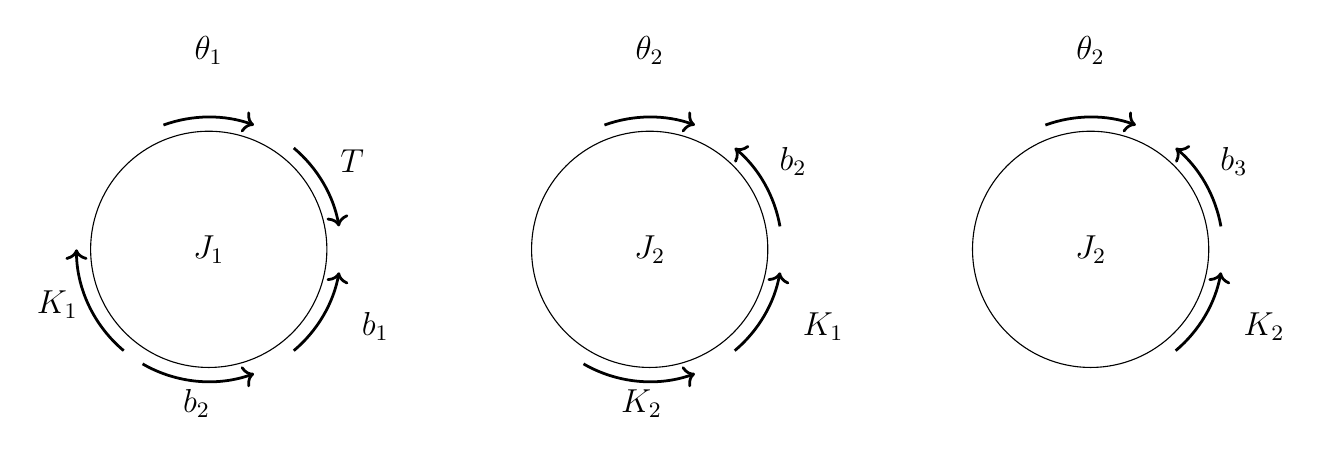
\begin{tikzpicture}[scale=1.4, every node/.style={font=\large}]

    % Circle for J1
    \node[circle, draw, minimum size=3cm] (inertia) at (0,0) {$J_1$};

    % theta1
    \draw[<-, line width=1pt] (70:1.2cm) arc[start angle=70, end angle=110, radius=1.2cm];
    \node at (0,1.8) {$\theta_1$};

    % torque
    \draw[->, line width=1pt] (50:1.2cm) arc[start angle=50, end angle=10, radius=1.2cm];
    \node at (1.3,0.8) {$T$};
    
    % b1
    \draw[->, line width=1pt] (310:1.2cm) arc[start angle=310, end angle=350, radius=1.2cm];
    \node[anchor=west] at (1.3,-0.7) {$b_1$};

    % b2
    \draw[->, line width=1pt] (240:1.2cm) arc[start angle=240, end angle=290, radius=1.2cm];
    \node[anchor=east] at (0.1,-1.4) {$b_2$};

    % k1
    \draw[->, line width=1pt] (230:1.2cm) arc[start angle=230, end angle=180, radius=1.2cm];
    \node[anchor=east] at (-1.1,-0.5) {$K_1$};
    
\begin{scope}[shift={(4,0)}]

    % Circle for J2
    \node[circle, draw, minimum size=3cm] (inertia) at (0,0) {$J_2$};

    % theta2
    \draw[<-, line width=1pt] (70:1.2cm) arc[start angle=70, end angle=110, radius=1.2cm];
    \node at (0,1.8) {$\theta_2$};

    % b2
    \draw[<-, line width=1pt] (50:1.2cm) arc[start angle=50, end angle=10, radius=1.2cm];
    \node at (1.3,0.8) {$b_2$};
    
    % k1
    \draw[->, line width=1pt] (310:1.2cm) arc[start angle=310, end angle=350, radius=1.2cm];
    \node[anchor=west] at (1.3,-0.7) {$K_1$};

    % k2
    \draw[->, line width=1pt] (240:1.2cm) arc[start angle=240, end angle=290, radius=1.2cm];
    \node[anchor=east] at (0.2,-1.4) {$K_2$};

\end{scope}
\begin{scope}[shift={(8,0)}]

    % Circle for J2
    \node[circle, draw, minimum size=3cm] (inertia) at (0,0) {$J_2$};

    % theta2
    \draw[<-, line width=1pt] (70:1.2cm) arc[start angle=70, end angle=110, radius=1.2cm];
    \node at (0,1.8) {$\theta_2$};

    % b3
    \draw[<-, line width=1pt] (50:1.2cm) arc[start angle=50, end angle=10, radius=1.2cm];
    \node at (1.3,0.8) {$b_3$};
    
    % k2
    \draw[->, line width=1pt] (310:1.2cm) arc[start angle=310, end angle=350, radius=1.2cm];
    \node[anchor=west] at (1.3,-0.7) {$K_2$};


\end{scope}
\end{tikzpicture}
\end{figure}

Torque balance on Inertia 1:
\[
T(s) - D_1 \theta_1 - D_2(\theta_1 - \theta_2) - K_1(\theta_1 - \theta_2) = J_1 s^2 \theta_1
\]
\[
T(s) - 3\theta_1 - 2(\theta_1 - \theta_2) - 4(\theta_1 - \theta_2) = 6s^2 \theta_1
\]
\[
T(s) - 3\theta_1 - 6\theta_1 + 6\theta_2 = 6s^2 \theta_1
\]
\[
T(s) - 9\theta_1 + 6\theta_2 = 6s^2 \theta_1
\]
\[
T(s) + 6\theta_2 = (6s^2 + 9)\theta_1 \quad \text{(1)}
\]

Torque balance on Inertia 2:
\[
- D_2(\theta_2 - \theta_1) - K_1(\theta_2 - \theta_1) - K_2(\theta_2 - \theta_3) = J_2 s^2 \theta_2
\]
\[
- 2(\theta_2 - \theta_1) - 4(\theta_2 - \theta_1) - 10(\theta_2 - \theta_3) = 3s^2 \theta_2
\]
\[
-6\theta_2 + 6\theta_1 -10\theta_2 + 10\theta_3 = 3s^2 \theta_2
\]
\[
-16\theta_2 + 6\theta_1 + 10\theta_3 = 3s^2 \theta_2
\]
\[
6\theta_1 + 10\theta_3 = (3s^2 + 16)\theta_2 \quad \text{(2)}
\]

Torque balance on Inertia 3:
\[
- K_2(\theta_3 - \theta_2) - D_3 \theta_3 = J_3 s^2 \theta_3
\]
\[
-10(\theta_3 - \theta_2) - 5\theta_3 = 1.5s^2 \theta_3
\]
\[
-10\theta_3 + 10\theta_2 - 5\theta_3 = 1.5s^2 \theta_3
\]
\[
10\theta_2 - 15\theta_3 = 1.5s^2 \theta_3
\]
\[
10\theta_2 = (1.5s^2 + 15)\theta_3 \quad \text{(3)}
\]

Substitute (3) into (2):
\[
6\theta_1 + 10\theta_3 = (3s^2 + 16)\left( \frac{(1.5s^2 + 15)\theta_3}{10} \right)
\]
\[
6\theta_1 + 10\theta_3 = \frac{(3s^2 + 16)(1.5s^2 + 15)}{10} \theta_3
\]
\[
6\theta_1 = \left( \frac{(3s^2 + 16)(1.5s^2 + 15)}{10} - 10 \right) \theta_3
\]

Substitute into (1):
\[
T(s) + 6\theta_2 = (6s^2 + 9)\theta_1
\]

\[
T(s) + 6\left( \frac{(1.5s^2 + 15)\theta_3}{10} \right) = (6s^2 + 9)\left( \frac{1}{6} \left( \frac{(3s^2 + 16)(1.5s^2 + 15)}{10} - 10 \right) \theta_3 \right)
\]

Simplify both sides:
\[
T(s) + \frac{9s^2 + 90}{10} \theta_3 = \left( \frac{(6s^2 + 9)((3s^2 + 16)(1.5s^2 + 15) - 100)}{60} \right) \theta_3
\]

Solve for \( \frac{\theta_3(s)}{T(s)} \):
\[
\frac{\theta_3(s)}{T(s)} = \frac{1}{\left( \frac{(6s^2 + 9)((3s^2 + 16)(1.5s^2 + 15) - 100)}{60} - \frac{9s^2 + 90}{10} \right)}
\]

Expand numerator:
\[
(3s^2 + 16)(1.5s^2 + 15) = 4.5s^4 + 45s^2 + 24s^2 + 240 = 4.5s^4 + 69s^2 + 240
\]
\[
(6s^2 + 9)(4.5s^4 + 69s^2 + 140) = 27s^6 + 414s^4 + 1230s^2 + 405s^4 + 621s^2 + 1260
\]
\[
= 27s^6 + 819s^4 + 1851s^2 + 1260
\]

Final expression:
\[
\frac{\theta_3(s)}{T(s)} = \frac{60}{27s^6 + 819s^4 + 1851s^2 + 1260 - 6(9s^2 + 90)}
\]
\[
\frac{\theta_3(s)}{T(s)}  = \frac{60}{27s^6 + 819s^4 + 1797s^2 + 720}
\]

\[
\boxed{\frac{\theta_3(s)}{T(s)} = \frac{60}{27s^6 + 819s^4 + 1797s^2 + 720}}
\]

% Problem 24
\newpage

\noindent\rule{\textwidth}{1pt}
\noindent\textbf{Problem 24} \hfill
\\ Determine the transfer function \(H(s) = \frac{\theta_3(s)}{T(s)}\) for the rotational system shown below.

\begin{figure}[!ht]
\centering
\resizebox{1\textwidth}{!}{%
\begin{tikzpicture}[scale=1.4, transform shape, font=\large]
   
   % ground and walls
    \draw[pattern=bricks] (6.6,-3) rectangle (8.3,-3.6); 
    \draw[pattern=bricks] (-2.3,-1.5) rectangle (-1.5,1.5);
    \draw[pattern=bricks] (16.3,-1.5) rectangle (17.1,1.5);

    % line
    \draw (-1.5,0) -- (0,0);   
    
    % j1
    \draw (0,0) ellipse (0.3cm and 1cm);  
    \draw (0,1) -- (3,1);                 
    \draw (0,-1) -- (3,-1);               
    \draw (3,1) arc[start angle=90, end angle=-90, x radius=0.3cm, y radius=1cm]; 
    \node at (1.7,0) {$1kg-m^2$};

     % j2
    \draw (10.6,0) ellipse (0.3cm and 1cm);  
    \draw (10.6,1) -- (13.6,1);                 
    \draw (10.6,-1) -- (13.6,-1);               
    \draw (13.6,1) arc[start angle=90, end angle=-90, x radius=0.3cm, y radius=1cm]; 
    \node at (12.3,0) {$2kg-m^2$};

    % fv1
    \pic [scale=1.35] at (3.25,0.5) {damper}; 
    \draw (7,0.5) -- (7,-0.6); 
    \node at (4.7,1.3) {$1 N \cdotp m\cdotp s/rad$};
    
    % fv2
    \pic [scale=0.9] at (13.8,0.5) {damper}; 
    \node at (14.7,1.4) {$1 N \cdotp m\cdotp s/rad$};

    % fv3
    \pic [scale=1.08, rotate=90] at (7.5,-3) {damper}; 
    \node at (9.2,-2.3) {$1\,\mathrm{N \cdotp m\cdotp s/rad}$};              

    % k1
    \pic [scale=1.85] at (3.25,-0.55) {coil spring};
    \node at (4.8,-1.2) {$1 N \cdotp m/rad$};

    % k2
    \pic [scale=1.85] at (7,0) {coil spring};
    \node at (8.7,0.8) {$1 N \cdotp m/rad$};

    % k3
    \pic [scale=1.2] at (13.9,-0.4) {coil spring};
    \node at (14.9,-1) {$1 N \cdotp m/rad$};
    
    % torque
    \draw[->, thick, color=cyan] (2,-1.3) arc[start angle=290, end angle=45, x radius=0.5cm, y radius=1.5cm];
    \node at (2,2) {$T$};
    
    % t2
    \draw[->, thick, color=cyan] (12.4,-1.3) arc[start angle=290, end angle=45, x radius=0.5cm, y radius=1.5cm];
    \node at (12.4,2) {$\theta_2$};

\end{tikzpicture}
}%
\end{figure}

\noindent\rule{\textwidth}{1pt}

\textbf{Given:}
\[
J_1 = 1,\quad J_2 = 2\ \text{(kg·m}^2\text{)} 
\]
\[
k_1 = 1,\quad k_2 = 1,\quad k_3 = 1\ \text{(N·m/rad)}
\]
\[
b_1 = 1\ \text{(between }J_1\text{ and mid node)},
\]
\[
b_3 = 1\ \text{(mid node to ground)}
\]
\[
b_2 = 1\ \text{(at }J_2\text{ to ground)}\ \text{(N·m·s/rad)}
\]
\[
T(t)\ \text{applied to }J_1 
\]
\[
\theta_1(t)\ \text{(at }J_1),
\qquad \theta_m(t)\ \text{(mid node)},
\qquad \theta_2(t)\ \text{(at }J_2)
\]


\textbf{Required:}
\[
H(s)=\frac{\theta_2(s)}{T(s)} .
\]

\textbf{Solution:}

Free Body Diagram

\begin{figure}[!ht]
\centering
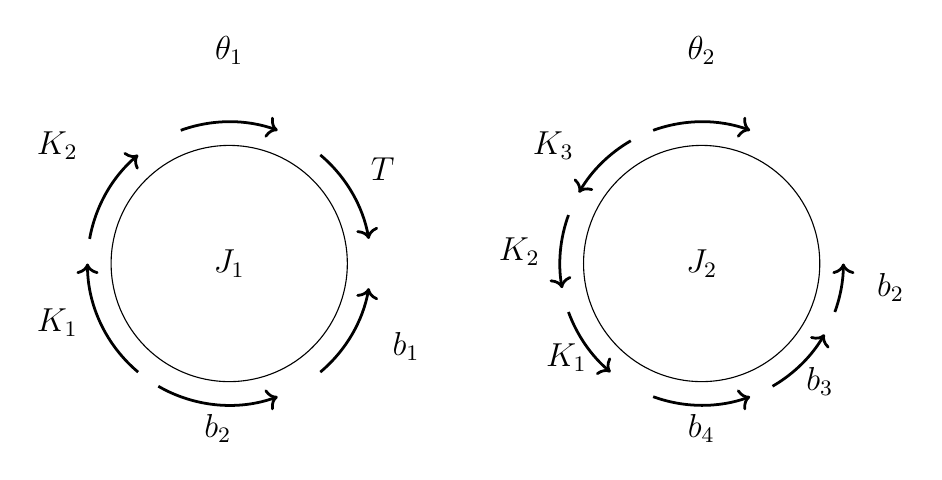
\begin{tikzpicture}[scale=1.5, every node/.style={font=\large}]

    % Circle for J1
    \node[circle, draw, minimum size=3cm] (inertia) at (0,0) {$J_1$};

    % theta1
    \draw[<-, line width=1pt] (70:1.2cm) arc[start angle=70, end angle=110, radius=1.2cm];
    \node at (0,1.8) {$\theta_1$};

    % torque
    \draw[->, line width=1pt] (50:1.2cm) arc[start angle=50, end angle=10, radius=1.2cm];
    \node at (1.3,0.8) {$T$};
    
    % b1
    \draw[->, line width=1pt] (310:1.2cm) arc[start angle=310, end angle=350, radius=1.2cm];
    \node[anchor=west] at (1.3,-0.7) {$b_1$};

    % b2
    \draw[->, line width=1pt] (240:1.2cm) arc[start angle=240, end angle=290, radius=1.2cm];
    \node[anchor=east] at (0.1,-1.4) {$b_2$};

    % k1
    \draw[->, line width=1pt] (230:1.2cm) arc[start angle=230, end angle=180, radius=1.2cm];
    \node[anchor=east] at (-1.2,-0.5) {$K_1$};

    % k2
    \draw[->, line width=1pt] (170:1.2cm) arc[start angle=170, end angle=130, radius=1.2cm];
    \node[anchor=east] at (-1.2,1) {$K_2$};
    
\begin{scope}[shift={(4,0)}]

    % Circle for J2
    \node[circle, draw, minimum size=3cm] (inertia) at (0,0) {$J_2$};

    % theta2
    \draw[<-, line width=1pt] (70:1.2cm) arc[start angle=70, end angle=110, radius=1.2cm];
    \node at (0,1.8) {$\theta_2$};
    
    % K3
    \draw[->, line width=1pt] (120:1.2cm) arc[start angle=120, end angle=150, radius=1.2cm];
    \node[anchor=west] at (-0.2,-1.4) {$b_4$};
    % b2
    \draw[->, line width=1pt] (160:1.2cm) arc[start angle=160, end angle=190, radius=1.2cm];
    \node at (1.6,-0.2) {$b_2$};

    % b3
    \draw[->, line width=1pt] (200:1.2cm) arc[start angle=200, end angle=230, radius=1.2cm];
    \node at (1,-1) {$b_3$};

    
    % k1
    \draw[->, line width=1pt] (300:1.2cm) arc[start angle=300, end angle=330, radius=1.2cm];
    \node[anchor=west] at (-1.4,-0.8) {$K_1$};

    % k2
    \draw[->, line width=1pt] (340:1.2cm) arc[start angle=340, end angle=360, radius=1.2cm];
    \node[anchor=west] at (-1.8,0.1) {$K_2$};

    % k3
    \draw[->, line width=1pt] (250:1.2cm) arc[start angle=250, end angle=290, radius=1.2cm];
    \node[anchor=east] at (-1,1) {$K_3$};


\end{scope}
\end{tikzpicture}
\end{figure}

Inertia 1:
\[
T(s) - K(\theta_1 - \theta_2) - D(\theta_1 - \theta_2) = J_1 s^2 \theta_1
\]
\[
T(s) - 2(\theta_1 - \theta_2) = s^2 \theta_1 \tag{1}
\]

Inertia 2:
\[
-K(\theta_3 - \theta_2) - D(\theta_3 - \theta_2) - K\theta_3 - D\theta_3 = J_2 s^2 \theta_3
\]
\[
-2(\theta_3 - \theta_2) - 2\theta_3 = 2s^2 \theta_3
\Rightarrow 2\theta_2 - 4\theta_3 = 2s^2 \theta_3 \tag{2}
\]

From (2):
\[
\theta_2 = \theta_3(s^2 + 2) \tag{3}
\]

Substitute (3) into (1):
\[
T(s) - 2(\theta_1 - \theta_3(s^2 + 2)) = s^2 \theta_1
\Rightarrow T(s) = \theta_1(s^2 + 2) - 2\theta_3(s^2 + 2)
\]

Solve for \( \theta_1 \):
\[
\theta_1 = \frac{T(s)}{s^2 + 2} + 2\theta_3 \tag{4}
\]

Substitute (4) into (3):
\[
\theta_2 = \theta_3(s^2 + 2)
\]

\[
T(s) = (\theta_1)(s^2 + 2) - 2\theta_2
= \left( \frac{T(s)}{s^2 + 2} + 2\theta_3 \right)(s^2 + 2) - 2\theta_3(s^2 + 2)
\]

\[
T(s) = T(s) + 2\theta_3(s^2 + 2) - 2\theta_3(s^2 + 2)
\Rightarrow T(s) = T(s)
\]

\[
2\theta_2 = 2s^2 \theta_3 + 4\theta_3
\Rightarrow \theta_2 = \theta_3(s^2 + 2)
\]

Substitute into (1):
\[
T(s) = \theta_1(s^2 + 2) - 2\theta_3(s^2 + 2)
\Rightarrow \theta_1 = \frac{T(s)}{s^2 + 2} + 2\theta_3
\]

\[
T(s) = \left( \frac{T(s)}{s^2 + 2} + 2\theta_3 \right)(s^2 + 2) - 2\theta_3(s^2 + 2)
\Rightarrow T(s) = T(s)
\]

\[
2\theta_2 = 2s^2 \theta_3 + 4\theta_3
\Rightarrow \theta_2 = \theta_3(s^2 + 2)
\]

From (1):
\[
T(s) = \theta_1(s^2 + 2) - 2\theta_2
\]
\[
T(s) = \left( \frac{T(s)}{s^2 + 2} + 2\theta_3 \right)(s^2 + 2) - 2\theta_3(s^2 + 2)
\Rightarrow T(s) = T(s)
\]

\[
\boxed{\frac{\theta_3(s)}{T(s)} = \frac{1}{s^4 + 5s^2 + 6}}
\]

% Problem 25
\newpage

\noindent\rule{\textwidth}{1pt}
\noindent\textbf{Problem 25} \hfill
\\ Determine the transfer function \(H(s) = \frac{\theta_o(s)}{T(s)}\) for the rotational system shown below.

\begin{figure}[!ht]
\centering
\resizebox{1\textwidth}{!}{%
\begin{tikzpicture}[scale=1.4, transform shape, font=\large]
   
   % ground and walls
    \draw[pattern=bricks] (1.1,-4) rectangle (2.5,-4.6); 
    \draw[pattern=bricks] (7.9,-4) rectangle (9.5,-4.6); 
    \draw[pattern=bricks] (-2.5,-1.5) rectangle (-3.3,1.5);
    \draw[pattern=bricks] (13.2,-1.5) rectangle (14.0,1.5);

    % j1
    \draw (0.3,0) ellipse (0.3cm and 1cm);  
    \draw (0.3,1) -- (3.3,1);                 
    \draw (0.3,-1) -- (3.3,-1);               
    \draw (3.3,1) arc[start angle=90, end angle=-90, x radius=0.3cm, y radius=1cm]; 
    \node at (1.9,0) {$6kg\cdot m^2$};

    % j2
    \draw (7.0,0) ellipse (0.3cm and 1cm);  
    \draw (7.0,1) -- (10.0,1);                 
    \draw (7.0,-1) -- (10.0,-1);               
    \draw (10.0,1) arc[start angle=90, end angle=-90, x radius=0.3cm, y radius=1cm]; 
    \node at (8.7,0) {$4kg\cdot m^2$};
    
    % fv1
    \pic [scale=1] at (-2.5,0) {damper};                
    \node at (-1.3,0.7) {$4\,\mathrm{N \cdotp m\cdotp s/rad}$};

    % fv2
    \pic [scale=1.1, rotate=90] at (8.7,-4) {damper}; 
    \node at (10.1,-3.2) {$2\,\mathrm{N \cdotp m\cdotp s/rad}$}; 

    % k1
    \pic [scale=1.5, rotate=90] at (1.8,-4) {coil spring};
    \node at (0.4,-2.5) {$5\,\mathrm{N \cdotp m/rad}$};

    % k2
    \pic [scale=1.65] at (3.65,0) {coil spring};
    \node at (5.2,0.6) {$3\,\mathrm{N \cdotp m/rad}$};

     % k3
    \pic [scale=1.5] at (10.3,0) {coil spring};
    \node at (11.7,0.6) {$6\,\mathrm{N \cdotp m/rad}$};
    
    % torque
    \draw[->, thick, color=cyan] (1.8,-1.3) arc[start angle=290, end angle=45, x radius=0.5cm, y radius=1.5cm];
    \node at (1.8,2) {$T$};

    % t2
    \draw[->, thick, color=cyan] (8.7,-1.3) arc[start angle=290, end angle=45, x radius=0.5cm, y radius=1.5cm];
    \node at (8.7,2) {$\theta_2$};

\end{tikzpicture}
}%
\end{figure}

\noindent\rule{\textwidth}{1pt}

\solutionheader
\textbf{Given:}
\[
J_1 = 6\ \mathrm{kg\cdot m^2},\quad J_2 = 4\ \mathrm{kg\cdot m^2} 
\]
\[
k_1 = 5,\ k_2 = 3,\ k_3 = 6\ \mathrm{N\cdot m/rad}
\]
\[
b_1 = 4,\ b_2 = 2\ \mathrm{N\cdot m\cdot s/rad}
\]
\[
T(t) \text{ applied to } J_1 
\]
\[
\theta_1(t),\ \theta_2(t)
\]

\textbf{Required:}
\[
H(s) = \frac{\theta_2(s)}{T(s)}
\]

\textbf{Solution:}

Free Body Diagram

\begin{figure}[!ht]
\centering
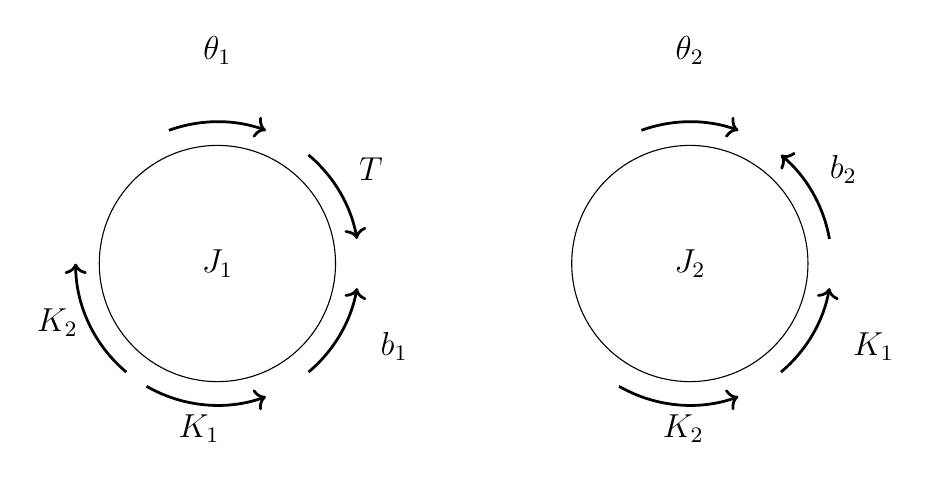
\begin{tikzpicture}[scale=1.5, every node/.style={font=\large}]

    % Circle for J1
    \node[circle, draw, minimum size=3cm] (inertia) at (0,0) {$J_1$};

    % theta1
    \draw[<-, line width=1pt] (70:1.2cm) arc[start angle=70, end angle=110, radius=1.2cm];
    \node at (0,1.8) {$\theta_1$};

    % torque
    \draw[->, line width=1pt] (50:1.2cm) arc[start angle=50, end angle=10, radius=1.2cm];
    \node at (1.3,0.8) {$T$};
    
    % b1
    \draw[->, line width=1pt] (310:1.2cm) arc[start angle=310, end angle=350, radius=1.2cm];
    \node[anchor=west] at (1.3,-0.7) {$b_1$};

    % k1
    \draw[->, line width=1pt] (240:1.2cm) arc[start angle=240, end angle=290, radius=1.2cm];
    \node[anchor=east] at (0.1,-1.4) {$K_1$};

    % k2
    \draw[->, line width=1pt] (230:1.2cm) arc[start angle=230, end angle=180, radius=1.2cm];
    \node[anchor=east] at (-1.1,-0.5) {$K_2$};
    
\begin{scope}[shift={(4,0)}]

    % Circle for J2
    \node[circle, draw, minimum size=3cm] (inertia) at (0,0) {$J_2$};

    % theta2
    \draw[<-, line width=1pt] (70:1.2cm) arc[start angle=70, end angle=110, radius=1.2cm];
    \node at (0,1.8) {$\theta_2$};

    % b2
    \draw[<-, line width=1pt] (50:1.2cm) arc[start angle=50, end angle=10, radius=1.2cm];
    \node at (1.3,0.8) {$b_2$};
    
    % k1
    \draw[->, line width=1pt] (310:1.2cm) arc[start angle=310, end angle=350, radius=1.2cm];
    \node[anchor=west] at (1.3,-0.7) {$K_1$};

    % k2
    \draw[->, line width=1pt] (240:1.2cm) arc[start angle=240, end angle=290, radius=1.2cm];
    \node[anchor=east] at (0.2,-1.4) {$K_2$};

\end{scope}
\end{tikzpicture}
\end{figure}

Torque balance on Inertia 1:
\[
T(s) - D_A \theta_1 - K_1 \theta_1 - D_B (\theta_1 - \theta_2) - K_2 (\theta_1 - \theta_2) = J_1 s^2 \theta_1
\]
\[
T(s) - (D_A + K_1)\theta_1 - (D_B + K_2)(\theta_1 - \theta_2) = J_1 s^2 \theta_1
\]
\[
T(s) - 7\theta_1 - 7(\theta_1 - \theta_2) = 6s^2 \theta_1
\]
\[
T(s) - 14\theta_1 + 7\theta_2 = 6s^2 \theta_1
\]
\[
T(s) + 7\theta_2 = (6s^2 + 14)\theta_1 \quad \text{(1)}
\]

Torque balance on Inertia 2:
\[
- D_C \theta_2 - (D_B + K_2)(\theta_2 - \theta_1) = J_2 s^2 \theta_2
\]
\[
- 6\theta_2 - 7(\theta_2 - \theta_1) = 5s^2 \theta_2
\]
\[
-13\theta_2 + 7\theta_1 = 5s^2 \theta_2
\]
\[
7\theta_1 = (5s^2 + 13)\theta_2 \quad \text{(2)}
\]

Substitute (2) into (1):
\[
T(s) + 7\theta_2 = (6s^2 + 14)\left( \frac{(5s^2 + 13)\theta_2}{7} \right)
\]
\[
T(s) + 7\theta_2 = \frac{(6s^2 + 14)(5s^2 + 13)}{7} \theta_2
\]
\[
T(s) = \left( \frac{(6s^2 + 14)(5s^2 + 13)}{7} - 7 \right) \theta_2
\]
\[
\frac{\theta_2(s)}{T(s)} = \frac{1}{\frac{(6s^2 + 14)(5s^2 + 13)}{7} - 7}
\]

\[
\frac{\theta_2(s)}{T(s)}= \frac{1}{\frac{30s^4 + 182s^2 + 182}{7} - 7}
\]

\[
\frac{\theta_2(s)}{T(s)}= \frac{1}{\frac{30s^4 + 182s^2 + 133}{7}}
\]

\[
\frac{\theta_2(s)}{T(s)}= \frac{7}{30s^4 + 182s^2 + 133}
\]

\[
\boxed{\frac{\theta_2(s)}{T(s)} = \frac{7}{30s^4 + 182s^2 + 133}}
\]